%% Copernicus Publications Manuscript Preparation Template for LaTeX Submissions
%% ---------------------------------
%% This template should be used for copernicus.cls
%% The class file and some style files are bundled in the Copernicus Latex Package, which can be downloaded from the different journal webpages.
%% For further assistance please contact Copernicus Publications at: production@copernicus.org
%% https://publications.copernicus.org/for_authors/manuscript_preparation.html


%% Please use the following documentclass and journal abbreviations for preprints and final revised papers.

%% 2-column papers and preprints
%\documentclass[journal abbreviation, manuscript]{copernicus} % default
\documentclass[gmd, preprint]{copernicus}


%% Journal abbreviations (please use the same for preprints and final revised papers)


% Advances in Geosciences (adgeo)
% Advances in Radio Science (ars)
% Advances in Science and Research (asr)
% Advances in Statistical Climatology, Meteorology and Oceanography (ascmo)
% Annales Geophysicae (angeo)
% Archives Animal Breeding (aab)
% Atmospheric Chemistry and Physics (acp)
% Atmospheric Measurement Techniques (amt)
% Biogeosciences (bg)
% Climate of the Past (cp)
% DEUQUA Special Publications (deuquasp)
% Drinking Water Engineering and Science (dwes)
% Earth Surface Dynamics (esurf)
% Earth System Dynamics (esd)
% Earth System Science Data (essd)
% E&G Quaternary Science Journal (egqsj)
% EGUsphere (egusphere) | This is only for EGUsphere preprints submitted without relation to an EGU journal.
% European Journal of Mineralogy (ejm)
% Fossil Record (fr)
% Geochronology (gchron)
% Geographica Helvetica (gh)
% Geoscience Communication (gc)
% Geoscientific Instrumentation, Methods and Data Systems (gi)
% Geoscientific Model Development (gmd)
% History of Geo- and Space Sciences (hgss)
% Hydrology and Earth System Sciences (hess)
% Journal of Bone and Joint Infection (jbji)
% Journal of Micropalaeontology (jm)
% Journal of Sensors and Sensor Systems (jsss)
% Magnetic Resonance (mr)
% Mechanical Sciences (ms)
% Natural Hazards and Earth System Sciences (nhess)
% Nonlinear Processes in Geophysics (npg)
% Ocean Science (os)
% Polarforschung - Journal of the German Society for Polar Research (polf)
% Primate Biology (pb)
% Proceedings of the International Association of Hydrological Sciences (piahs)
% Safety of Nuclear Waste Disposal (sand)
% Scientific Drilling (sd)
% SOIL (soil)
% Solid Earth (se)
% The Cryosphere (tc)
% Weather and Climate Dynamics (wcd)
% Web Ecology (we)
% Wind Energy Science (wes)


%% \usepackage commands included in the copernicus.cls:
%\usepackage[german, english]{babel}
\usepackage{tabularx}
\usepackage{tablefootnote}
%\usepackage{datetime2}  % \DMTnow
\usepackage[en-GB]{datetime2} % \usepackage[en-GB,en-US]{datetime2}
\DTMlangsetup[en-GB]{ord=raise,abbr,monthyearsep={,\space}}
% https://www.dickimaw-books.com/faq.php?itemlabel=datetime2adjustregional
%\usepackage{hyperref}
%\usepackage{cancel}
%\usepackage{multirow}
%\usepackage{supertabular}
%\usepackage{algorithmic}
%\usepackage{algorithm}
%\usepackage{amsthm}
%\usepackage{float}
%\usepackage{subfig}
%\usepackage{rotating}


%% define user commands
\newcommand{\mycomment}[1]{}
% autoref capitalisation
% https://tex.stackexchange.com/questions/34155/autoref-does-not-capitalize-initial-character-in-sentence-when-referencing-labe

% Define colours to capture author contributions
\def\cred#1{{\color{red}#1}}
\def\cblue#1{{\color{blue}#1}}

\begin{document}

\title{The Coupled Model Intercomparison Project (CMIP): Reviewing project history, evolution and future}
\mycomment{
was: The Coupled Model Intercomparison Project phase 6 (CMIP6): A review of project evolution and future
Pete G alternate: The Coupled Model Intercomparison Project phase 6 (CMIP6) made possible by an evolution of project implementation
Jiwoo alternate: The Coupled Model Intercomparison Project (CMIP): a review of project history, evolution and future
}

% \Author[affil]{given_name}{surname} % Author {first initial.}{last}
\Author[1]{Paul J.}{Durack} % ORCID 0000-0003-2835-1438
\Author[1]{Karl E.}{Taylor} % 0000-0002-6491-2135
\Author[1]{Peter J.}{Gleckler} % 0000-0003-2816-6224
\Author[2]{Matthew}{Mizielinski} % 0000-0002-3457-4702
\Author[3]{Daniel}{Ellis} % 0000-0001-6733-7028
\Author[1]{Jiwoo}{Lee} % 0000-0002-0016-7199
\Author[1]{Curt}{Covey} % 0000-0002-0016-7199
\Author[30]{others please}{add yourselves - will alphabetically reorder authors once final}
% \affil % Affiliations
\affil[1]{Program for Climate Model Diagnosis and Intercomparison (PCMDI), Lawrence Livermore National Laboratory (LLNL), Livermore, California, USA}
\affil[2]{Met Office Hadley Centre, Exeter, UK}
\affil[3]{CMIP International Project Office (CMIP-IPO), Oxfordshire, UK}
\affil[30]{Affiliation, location, country}

%% The [] brackets identify the author with the corresponding affiliation. 1, 2, 3, etc. should be inserted.

%% If an author is deceased, please mark the respective author name(s) with a dagger, e.g. "\Author[2,$\dag$]{Anton}{Smith}", and add a further "\affil[$\dag$]{deceased, 1 July 2019}".

%% If authors contributed equally, please mark the respective author names with an asterisk, e.g. "\Author[2,*]{Anton}{Smith}" and "\Author[3,*]{Bradley}{Miller}" and add a further affiliation: "\affil[*]{These authors contributed equally to this work.}".

\correspondence{Paul J. Durack (durack1@llnl.gov)}
\runningtitle{MIP: evolution and future}
\runningauthor{Durack et al.}


\received{}
\pubdiscuss{} %% only important for two-stage journals
\revised{}
\accepted{}
\published{}

%% These dates will be inserted by Copernicus Publications during the typesetting process.

\firstpage{1}
\maketitle


\begin{abstract}
\cred{Rewrite once other sections drafted}

   The CMIP6 project was the most expansive and ambitious Model Intercomparison Project (MIP) to date. Project planning began in 2013, with the first data available in 2018, and new data publication continues today. Over the planning to delivery period, the project grew from 21 to 26 MIPs and from around 190 to 322 experiments defined across them, providing comprehensive coverage of contemporary climate science. Project contributors, primarily modelling groups, also grew considerably in the latest phase, with 45 institutions representing 24 countries providing climate model simulation data to the project. Now that CMIP6 is nearing completion, we review its status, evolution over more than a decade of project planning and delivery, and opportunities and plans for future phases.

\cred{
\begin{itemize}
  \item Project grew beyond the scope of Eyring et al., 2016
  \item Phases: planning 2013-2017, operational 2018-present 
  \item Realized potential of distributed community MIPs
  \item Built long-standing goodwill with contributors and culture of sharing data: facilitating groups by providing compute time to run simulations; tools to aid data creation to meet formats; developing hosting solutions that allowed collation and dissemination of contributions; generating a project that allows individual contributions to be uniquely identified and feed into national and international/IPCC assessments, whilst preserving identities to ensure recognition is received
  \item Realized the potential of open-access data enabling science discovery and reproducibility
  \item CMIP6 in context with past
  \item CMIP6Plus and evolution planning underway
  \item Coordinated research has led to the development of a common language and nomenclature, enabling an international collaboration targeting the same scientific question with a myriad of modelling approaches following standard experimental and output protocols enabling broad data dissemination and use
  \item History has led to a community pile-on as the MIP standards developed from AMIP1 onward have facilitated scientific collaboration
  \item Economies of scale - set formats/infrastructure once, contribute science multiple times
  \item As MIP momentum has built, the total number of activities and the total number of experiments have grown, reflecting enhanced coordination and community buying into shared and standardized practices
  \item Aspiration is to guide infrastructure development through logic that enables the more and more comprehensive model and observational outputs to be uniquely and unambiguously identified, facilitating MIP contributors to generate and downstream data users to access and use these data
  \item VALE Larry Gates
\end{itemize}
} %% end\cred

\cred{
Yet to incorporate all Peter G edits from \href{https://docs.google.com/document/d/1l9e0kBbXHG55jFroicRbM-_gaRhTVulMr_F6S3aLQGQ/edit}{google doc}
}

%Planned submission Friday 25 October 2024.

\cred{Co-authors to engage}
\textbf{Jiwoo} (Shared - Coordinated evaluation), \textbf{Martina S} (Data citation), \textbf{Guillaume L/Atef B.-N.} (Data errata), \textbf{David H./Eric G.} (Model (and data) documentation).
\textbf{Dean W.} (ESGF), \textbf{Bryan L.} (ESGF), ESGF-XC membership?.
\textbf{CMIP Panel}: Jerry M., Ron S.; Broader panel.
\textbf{WIP Panel}: Bryan L., Balaji, ?; Broader panel past and present.

{Compiled: \DTMnow}

\end{abstract}

\copyrightstatement{TEXT} %% This section is optional and can be used for copyright transfers.


\introduction  %% \introduction[modified heading if necessary]
\cred{Rewrite once other sections drafted}

The Model Intercomparison Project (MIP) concept, a well-worn nomenclature in climate science \cred{\textbf{(a few REFs)}}, has existed for many decades. Among other things, the MIP era has delivered two critical advancements to climate science. The first, that modelling groups contributing to any particular MIP have agreed to make their model output available to be scrutinized by the research community. Before the advent of MIPs, this was generally not the case, as model analysis was typically performed by individual modelling groups or close collaborators \cred{\textbf{(a few REFs)}}. The second, that contributing to a MIP means agreeing to adhere to a defined experimental design, meaning simulation data could be directly compared.

The acronyms of the Coupled Model Intercomparison Project (CMIP) and Intergovernmental Panel on Climate Change (IPCC) are interchangeably referenced by scientists, stakeholders, and policymakers to refer to the latest climate-model-based science. The MIPs further inspired international effort coordination, leading to considerable science collaboration that has enabled breakthroughs, including the building consensus that human influence is "\textit{unequivocal}" in driving the observed climate changes we are experiencing today \citep{eyring_human_2021}. More comprehensive international coordination has marked their development as a way to systematically evaluate observed climate changes, generate plausible future projections driven by varying futures of human development, and assess the fidelity of global climate models (GCMs) and Earth System Models (ESMs) to reproduce past changes and gauge their responses and sensitivities to realistic and idealised climate forcing. The multi-model approach to climate change assessment is now routine, with documented and reproducible experimental protocols and forcing datasets facilitating standardized simulations that can be directly compared across models and with observations to ascertain forced signal from noise and identify robust model responses versus outliers and anomalies that are not representative of our best estimates of the real world.

To provide context for the most recent phase (CMIP6) and the planning of the project’s future, in this paper we discuss a variety of efforts dating back to the MIP origins, and how they contributed to making climate community collaboration what it is today. Many of the steps taken were initiated by small teams or individuals, and while evidence of this history is scattered in literature, here we attempt to bring them together to tell a coherent story of how CMIP got to where it is today. Our emphasis details the pragmatics of what it took to progressively scale efforts up, most recently delivering CMIP6, thus this paper describes the evolution of how the MIPs were implemented and the coordinated efforts to establish a minimal infrastructure to make that possible. In \autoref{sec:cmip6InContext} we discuss MIP phases from 1990 to 2015. In \autoref{sec:cmip6ProjectDesign} we highlight the CMIP6 experimental design, and in \autoref{sec:CMIPSupportingOrgsAndInfra} the supporting organizations and infrastructure, \autoref{sec:CMIP6SupportingProjects} describes CMIP6 supporting projects, \autoref{sec:CMIP6Completion} CMIP6 completion and next steps, and conclusions in \autoref{sec:Conclusions}.

\mycomment{
Mention CMIP6 Community MIPs - mentioned in CMIP5 section.
% Homogenize
https://docs.google.com/document/d/1Bxu2djLsB0blUUjr4qtwNpZWqMFXkTQRY8kOR_EJvlA/edit?skip_itp2_check=true&pli=1
}


\section{CMIP6 in context with the past}
\label{sec:cmip6InContext}

CMIP6 is the latest in a long history of internationally coordinated climate modelling research projects. The activities grew out of self-organizing communities that built collaborations around science questions and the recognition that systematic multi-model evaluation was needed to build confidence in climate models as effective tools for climate change prediction. The following section provides context around the preceding activities leading to the latest phase.

\cred{fold in pre-FANGIO history back to 1982 from \citep{ellingson_atmospheric_2016}, with 1984 the date noted when a GCM intercomparison was called for by DOE, a full 5-years before PCMDI/AMIP}

\mycomment{
1955-65: Establishment of Atmospheric General Circulation Modelling
http://pne.people.si.umich.edu/sloan/1955_65.html

Some notes from Curt C for AMIP and CMIP1/2 sections

Line 96: It's misleading to call AMIP runs "atmosphere-only." They also included an interactive land surface. In some cases it was very simple (e.g. Budyko bucket) but in all cases it needed to interact with the atmosphere.

Line 104: AMIP stored a time series of monthly means (120 of them for the 10-year AMIP1 period)--not just "climatological annual mean data."

Lines 16-24: Misleading intro to Section 2.2. "In parallel, work continued . . ." implies AOGCMs were developed alongside AMIP. Actually "The first attempts at coupling atmospheric and oceanic models were carried out during the late 1960s and early 1970s (Manabe and Bryan, 1969; Bryan et al., 1975; Manabe et al., 1975)." (IPCC 4AR, Section 1.5.3) Also, saying "climate change cannot be fully simulated without proper considerations of interactions with other major systems such as ocean" is too weak. We need to clearly point out that AMIP runs, with SST and seaice fixed, cannot simulate future global warming--or past global climate changes in which SSTs are poorly known.

Lines 39 and 54: Were "pdcntrl" and "picntrl" runs really different in practice?

Line 71: Add ". . . for most variables" to ". . . time-averaged quantities were collected."
}

\subsection{Atmospheric Model Intercomparison Project phases (AMIP1/2)}
\label{sec:amip1And2}
Intercomparison of the results from different atmospheric model simulations focused on predicting the near-term weather (numerical weather prediction) began soon after the first large scale atmospheric models were developed in the 1950s, with the Working Group on Numerical Experimentation (WGNE) coordinating these activities since the early 1970s \citep{gates_ams_1992}. The first internationally coordinated climate model experimentation occurred in the late 1980s, scientifically focused on cloud feedbacks in the Feedback ANalysis of GCMs and In Observations (FANGIO) project and contributions from 19 unique atmospheric model configurations \citep{cess_methodology_1988, cess_interpretation_1989, cess_intercomparison_1990, cess_first_1991}. The nascent community success quickly expanded into the first phase of the Atmospheric Model Intercomparison Project (AMIP, \citet{gates_amip_1992}, hereafter referred to as AMIP1), which was organized under the purview of WGNE for the World Climate Research Programme (WCRP) to help identify and ultimately reduce systematic errors in atmospheric models. The acronym AGCM (Atmospheric General Circulation Model) was coined to define model configurations for the project. AMIP1 augmented total atmospheric model configurations to 27, more definitively documenting the atmosphere-only experimental protocols, including providing standardized "forcing" sea surface temperature (SST) and sea-ice boundary conditions for the 1979-1988 period, in addition to recommended solar constant (1365 W m\textsuperscript{-2}) and carbon dioxide concentrations (345 ppm) \citep{gates_amip_1991}. The project expanded the required model output from simple global and zonal means in FANGIO to climatological annual mean data in three dimensions. For many participating models, AMIP1 was the first opportunity to run their model longer than one annual cycle, with computer time provided by the Program for Climate Model Diagnosis and Intercomparison (PCMDI; see \autoref{sec:CMIPSupportingOrgsAndInfra}) allowing for 10-year integrations. Early AMIP1 results were incorporated into the IPCC First Assessment Report (FAR) \citep{gates_validation_1990}. As the second phase (AMIP2) was being planned, including an improved experimental design and updated forcing \citep{liang_pcmdi_1997, taylor_pcmdi_2000}, considerable efforts were made to leverage AMIP analysis in the IPCC Second Assessment Report (SAR) \citep{gates_climate_1996}, with a focus on assessing mean errors and multi-model consistency across the archive \citep{gates_amip_1995}. \cred{the details of AMIP2 are light, can we augment - Pete G?}


\subsection{Coupled Model Intercomparison Project phases (CMIP1/2/2+)}
\label{sec:cmip1And2And2Plus}
In parallel, work continued at modelling centres to expand model complexity to incorporate a dynamic ocean, amongst other climate system components. Acknowledging that climate change can not be fully simulated without proper considerations of interactions with other major systems such as ocean, the effort to couple additional components to the atmosphere-centric models led to the creation of the WCRP Steering Group on Global Coupled Models (SGGCM), established in November 1990. Over the following years, the activity entrained oceanographers working in parallel on ocean model development, encapsulated by work hosted by the WCRP CLImate VARiability and Predictability (CLIVAR) project (the CLIVAR Working Group on Ocean Model Development (WGOMD) was subsequently established in 1998). The growing coordination led to the Coupled Model Intercomparison Project (CMIP) acronym being defined and the first phase, CMIP1, being determined after a workshop was held at Scripps Institution of Oceanography in October 1994 \citep{meehl_global_1995}. The acronym AOGCM (Atmosphere-Ocean General Circulation Model) was coined to define model configurations for this project. CMIP1 was focused on collecting data and documenting features of AOGCMs of present-day fixed climate (pdcntrl; see \autoref{tab:tabAppA1-MIPExperiments} for more details). The new community MIP data resource led to considerable community attention and evaluation of the building archive \citep{villwock_6th_2003, lambert_cmip1_2001, raisanen_co2-induced_2001}. In September 1995, the CLIVAR decadal-centennial variations and anthropogenic climate change (DecCen/ACC) Numerical Experimentation Group (NEG-2) was established, which defined an ambitious program of modelling studies, including CMIP \citep{villwock_what_1996, coughlan_report_1996}. The project gathered momentum quickly, with a broad expansion in community-proposed diagnostic subprojects leveraging science insights from the growing archive, and a second phase, CMIP2, was planned and announced in January 1997 \citep{meehl_intercomparison_1997, meehl_coupled_2000}. CMIP2 broadened the science remit, expanding the focus to include a pre-industrial ($\sim$1860) control (picntrl) and climate sensitivity experiments with CO2 increasing at 1\% per year (1pctto2x, 1pctto4x) \citep{villwock_6th_2003, meehl_cmip_2003}. In parallel to the CMIP growth, there was a recognition that coordinating this activity required a dedicated working group. In April 1997 the WCRP Working Group on Coupled Modelling (WGCM) was created at a CLIVAR SSG meeting in Washington DC, reconstituting CLIVAR NEG-2 to meet the growing project needs \citep{detemmerman_clivar_1997} and bringing the project structure and hierarchy inline with what we have in place today. Like their AMIP counterparts, the CMIP model output saw strong attention, with early results also included in the IPCC SAR \citep{gates_climate_1996} and IPCC Third Assessment Report (TAR) \citep{mcavaney_model_2001}. With the growing interest in available model data, a recognition was made that the standard output collected to date was only a small subset of model data produced. For the preceding phases, time-averaged quantities were collected. In contrast, the time-varying monthly mean information available for a handful of fields (surface temperature, precipitation, and sea level pressure) enabled far broader scientific investigations. Recognizing this opportunity, an augmented phase CMIP2+ was identified and announced in May 2000 \citep{villwock_6th_2003, meehl_cmip_2003, meehl_overview_2005}, with a subset of CMIP1/2 contributing modelling groups augmenting their existing data contributions with considerably more variable and time coverage, including daily data if available \citep{achutarao_pcmdi_2004}.

CMIP2+ enabled research beyond the scope possible with CMIP1 and CMIP2, most notably a comprehensive appraisal of climate models for the US Department of Energy \citep{achutarao_pcmdi_2004}. But it soon became apparent that both contributors and users would greatly benefit from detailed model output specifications--including uniform data formats and standard variable names, units, dimensions, etc. At the same time the culture of climate-change research had evolved to make open data sharing an expected practice. These two considerations led to the next phase of CMIP, which PCMDI officially agreed support and host, and endorsed by the WGCM (representing contributing modelling groups) in October 2003.

\mycomment{
Curt C to provide a sentence or two about the dramatic growth of the registered subprojects that had been the standard engagement way in AMIP1/2, CMIP1/2 and how that
led to the opening up of the CMIP3 archive to open-access 85 FTP, and no registered subprojects? - If I have that right?

WGOMD establishment after WGCM-2 in Melbourne Oct 1998 - see https://eprints.soton.ac.uk/30149/1/040_wgcm4.pdf#Page=9 /sect3.5 also JSC-21 also see https://www.wcrp-climate.org/modelling-wgcm-publications
CMIP1/2/2+ announcement emails for timing - https://web.archive.org/web/20040827091054/http://www-pcmdi.llnl.gov/cmip/
Also PMIP 1991 - prescribed SSTs AGCMs \citep{braconnot_paleoclimate_2011} \textbf{(Karl to help here)}
Also AMIP2 proceedings, Gleckler et al 2005 - https://pcmdi.llnl.gov/mips/amip/amip2_workshop_proceedings.pdf#page=11 - https://www.osti.gov/biblio/15014509
And Potter 1999 - new strategy beyond AMIP - https://www.osti.gov/biblio/791127
Also Meehl 2019 https://www.wcrp-climate.org/images/AGU2019/presentations/Symposium/11-Meehl_WCRP40.pdf
}


\subsection{Coupled Model Intercomparison Project phase 3 (CMIP3)}
\label{sec:cmip3}
The considerable growth in coordinated MIPs continued throughout the early 2000s and led to the development of what became known as the third phase CMIP3 \citep{meehl_wcrp_2007}. In the early stages, activities that came to define the project were more identified by discrete subprojects, targeting science questions of ocean realism in comparison to observations \citep{orr_ocean_1999, dutay_evaluation_2002, dutay_evaluation_2004} and climate change detection and attribution research targeting the "historical" period \citep{hegerl_20c3m_2003}. Subsequently, many of the initial activities evolved into a more coordinated collection of experiments, which entrained an even more significant number of contributing modelling groups. The project saw a step-change across numerous facets, driven by growing and emerging science themes and an increasing appetite by a growing community to access these model data. All contributing models were coupled, simulating the atmosphere, ocean, sea-ice, and, in some cases, the first dynamic land components. By this phase, the flux adjustment, used by many CMIP1/2 contributing models, was largely unnecessary for most contributing AOGCM configurations \citep{durack_ocean_2012}. There was also a dramatic scientific expansion from the fixed pre-industrial control (picntrl) and idealized 1 percent compounding CO2 (1pctto2x, 1pctto4x) CMIP1/2 experiments to include for the first time a "Twentieth-century" simulation (20C3M; $\sim$1860-1999), extending from the mid-1800's through until the year 2000, and directly comparable to the growing observational record \citep{meehl_wcrp_2007}. The 20C3M experiment, along with parallel twenty-first century future projection simulations as documented in the Special Report on Emission Scenarios (SRES; 2000-2100; \citet{nakicenovic_summary_2000}) was a step-change for CMIP, for the first time providing model data that could be directly compared to the growing observational datasets, and outlining a project design that would be replicated to great effect in subsequent phases (to become ScenerioMIP in CMIP6). Partial motivation for the 20C3M experiment was to address the growing science around climate change detection and attribution \citep{santer_detection_1996-1, hegerl_20c3m_2003} a research focus that was rapidly expanding since the "..\emph{discernable} human influence on global climate" statement was published in the IPCC SAR \citep{santer_detection_1996}. The explicit recognition that unforced model internal variability needed to be better understood had also been identified by this stage, and multi-member ensembles (or runs) were encouraged to enable variability quantification \citep{meehl_wcrp_2007}. The project also began incorporating community science, parallel to official CMIP experiments. Notable communities, the nascent Cloud Feedback MIP (CFMIP) established in 2003, which had the single instantaneous CO2 doubling (2xco2) and slab ocean (slabcntl) experiments (also see \autoref{tab:tabAppA1-MIPExperiments}) \citep{mcavaney_cloud_2003, webb_cloud_2017} incorporated as part of the official CMIP3 experiment suite, in addition to Paleoclimate MIP phase 2 (PMIP2) which had been operating in parallel to the A/CMIP phases since 1991 \citep{villwock_6th_2003, braconnot_paleoclimate_2011}. Like their A/CMIP counterparts, CMIP3 model output saw even more attention than previous phases. These results, in addition to the body of literature that current and earlier phases of model simulation archives had facilitated, were prominently featured in the IPCC Fourth Assessment Report (AR4; \citet{randall_climate_2007}), which itself received the 2007 Nobel Peace Prize \citep{kerr_nobel_2007}.

\mycomment{
CLIVAR MIPs list circa 2005 - lots ~30
http://web.archive.org/web/20050319232556/http://www.clivar.org/science/mips.htm
This omits the CMIP Coordinated Experiment focus which were all announced in 2002 - https://web.archive.org/web/20040827091054/http://www-pcmdi.llnl.gov/cmip/ - subsequently known as CMIP3
Also https://pcmdi.llnl.gov/mips/cmip/ann_20c3m.html
Also PCMDI provided disks to modelling groups who copied data and posted them back - Meehl et al., 2003
Meehl & Hibbard, 2007: A STRATEGY FOR CLIMATE CHANGE STABILIZATION EXPERIMENTS WITH AOGCMs AND ESMs https://www.agci.org/wp-content/uploads/imported-files/2022/07/06S1_WhitePaper.pdf
C4MIP ~2002 https://web.archive.org/web/20040804013119/http://www.c4mip.cnrs-gif.fr/protocol.html
}


\subsection{Coupled Model Intercomparison Project phase 4 (CMIP4)}
\cred{Jerry M, and Ron S is this representative of reality?}
While no formal phase was identified CMIP4, some CMIP3 follow-on simulations focused on climate change detection and attribution, specifically single-forcing experiments that held all but one of the 20C3M forcings fixed, were undertaken by several modelling groups. However, these were never formally contributed to a managed multi-model CMIP archive \citep{stouffer_cmip5_2017}. The early effort was a precursor to the CMIP6 Detection and Attribution Model Intercomparison Project (DAMIP; \citet{gillett_detection_2016}), building off early work focused on resolving the regional patterns of greenhouse gas and sulphate aerosol forcing \cite{taylor_response_1994, santer_towards_1995, hegerl_optimal_2000, gillett_detecting_2002, hegerl_20c3m_2003}. As planning began for the experiments targeting the next IPCC Fifth Assessment (AR5), aligning the CMIP and the IPCC report phases was an additional motivation to skip the CMIP4 identifier. This additionally also avoided unnecessary confusion with the developing coordinated carbon-cycle modelling activities, with the Coupled Climate-Carbon Cycle Model Intercomparison Project (C4MIP) an active collaborative project of the WGCM and the International Geosphere-Biosphere Programme (IGBP) that had been running in parallel to the prior CMIP phases \citep{fung_full-form_2000, cox_modelling_2002, friedlingstein_climatecarbon_2006}. C4MIP was one of numerous parallel efforts leveraging science coordination nurtured by the growing MIP community.
\mycomment{
CMIP4 comment - https://www.wcrp-climate.org/images/modelling/WGCM/WGCM17/WGCM17_report.pdf#Page=8
}


\subsection{Coupled Model Intercomparison Project phase 5 (CMIP5)}
\label{sec:cmip5ProjectDesign}
The marked expansion of activities over preceding decades and an ever-expanding data user base led to a considerable project augmentation for its fifth phase (CMIP5). By this stage, many climate research subcommunities had identified MIPs as an effective way to scientifically collaborate, addressing the dual purposes of answering scientific questions through coordinated experimentation and identifying opportunities for model improvement by identifying consistent errors and biases across the multi-model ensembles. The developing data standards and delivery infrastructure also considerably aided collaboration (see \autoref{sec:CMIPSupportingOrgsAndInfra}), easing access to obtaining and using CMIP output. Planning for the project began in mid-2006 at an Aspen Global Change Institute session which collated representatives across physical climate science, biogeochemistry, impacts and adaptation, and integrated assessment modelling, which laid out needs for near-term and longer-term projection experiments \citep{meehl_introduction_2011}. By CMIP5, the core experiments had been identified, with CMIP core simulations AMIP, piControl, historical (20C3M), 1pctCO2, and an instantaneous CO2 quadrupling experiment (abrupt4xCO2) included, targeting model behaviour assessment and climate sensitivity. In addition, the success and attention of the future-focused SRES projections in CMIP3 led to an augmentation of four next-generation Representative Concentration Pathway (RCP) scenarios being defined \citep{moss_next_2010}. The importance of the carbon cycle through land and ocean biogeochemistry had also been recognized, which led to several experiments being included forced with CO2 emissions (rather than the imposed atmospheric concentrations of the preceding phases) which depended on Earth System Model (ESM) configurations to contribute \citep{hibbard_strategy_2007,meehl_introduction_2011}.

By 2011, the CMIP5 project design evolution already reflected the more formal MIP structure defined in the following phase (see \autoref{sec:cmip6ProjectDesign}). The CMIP5 "core" experiment set included the diagnostic piControl, AMIP, 20c3m/historical targeting model behaviours, and the 1pctCO2 and abrupt4xCO2 experiments evaluating climate sensitivity, mirroring the CMIP6 "DECK", with the projected future scenarios rcp45 and rcp85 also included \citep{stouffer_cmip5_2011}. The second tier included additional projected future scenarios rcp26 and rcp60 (precursors to ScenarioMIP experiments in CMIP6) \citep{hibbard_primer_2011}, CFMIP follow on experiments including patterned SST experiments sst2030, amip4xCO2, amipFuture, amip4K and along with the aquaplanet experiments aquaControl, aqua4xCO2 and aqua4K \citep{bony_cfmip_2011}, PMIP follow-on paleoclimate experiments included midHolocene, last glacial maximum (lgm) and past1000 \citep{braconnot_paleoclimate_2011}. The project also included experiments targeting short-lived climate forcers sstClimAerosol and sstClimSulfate \citep{boucher_climate_2011}, precursors to CMIP6 AerChemMIP, and the carbon-cycle focused experiments esmrcp85, esmFixClim1, esmFixClim2, esmFdbk1 and esmFdbk2 \citep{friedlingstein_climate-carbon_2011}, precursors to CMIP6 C4MIP. The addition or near-term or initialized prediction experiments was also new to CMIP, with these short-running experiments focused on predicting climate states from the next few years through to a couple of decades \citep{doblas-reyes_cmip5_2011}, identified by the decadalXXXX and noVolcXXXX experiments which in practice worked both in hindcast (back to 1959) and near-term future (to 2015), precursors to the CMIP6 DCPP activity.

\mycomment{
Map CMIP5 experiments to CMIP6 MIPs
https://github.com/PCMDI/CMIP5_CVs/blob/main/src/writeJson.py
https://docs.google.com/document/d/1bUwK6G_fVZO53UjLZbQUOuBP47PsT8lqKKhL1pjRnKg/edit
}


% all figures and data should live in standalone github repo
\begin{figure}
    \centering
    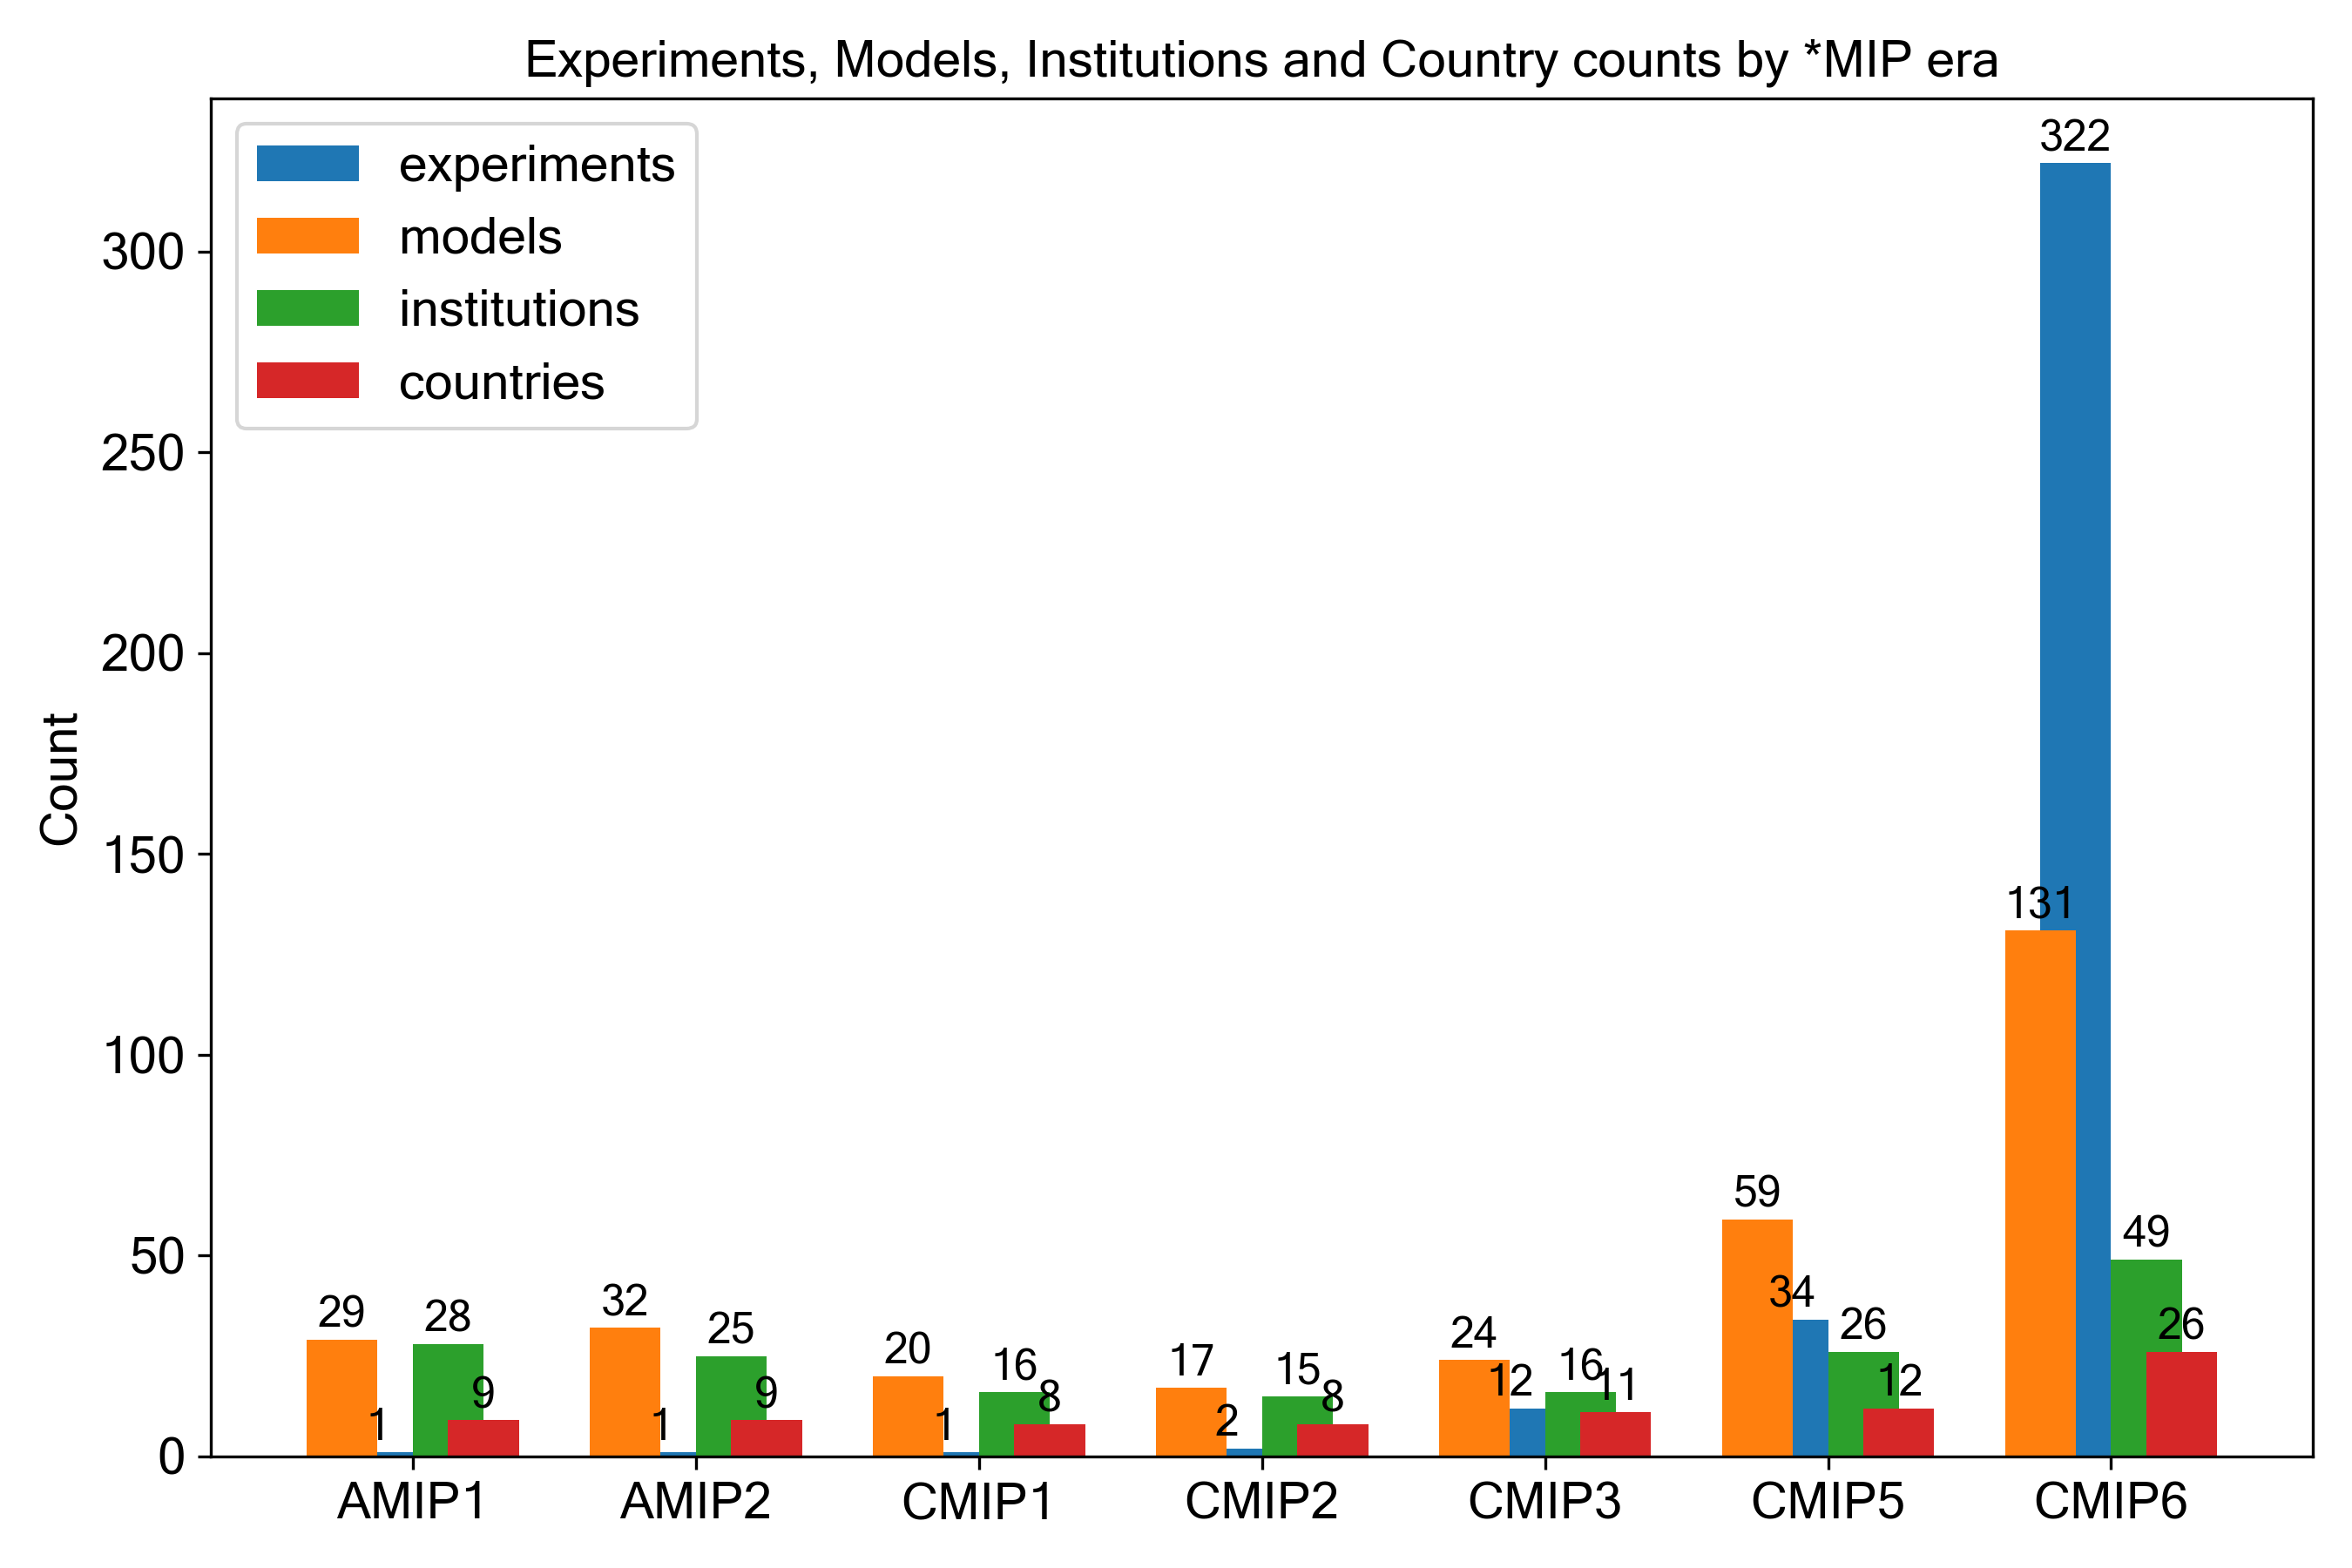
\includegraphics[width=1\linewidth]{230512T112843_MIPEvolution-Counts.png}
    \caption{Experiments, models, institutions, and countries contributing to completed Model Intercomparison Project (MIP) phases, from 1989 to today. The project's growth over the most recent phase reflects a growing community appetite for the latest climate data to inform decision-making, a distant evolution from the climate science origin of AMIP1. See \autoref{tab:tabAppA1-MIPExperiments} for an expansion of the experiment lists}
    \label{fig:fig1-MIPGrowth}
\end{figure}

%https://tex.stackexchange.com/questions/343028/vertical-centering-of-all-columns-in-tabularx-environment 
\begin{table*}[htp]
\renewcommand{\arraystretch}{1.5}
\scriptsize
\centering
\caption{The Model Intercomparison Projects (MIPs), through time}
\resizebox{\textwidth}{!} {
\begin{tabularx}{0.9\textwidth} {
  | >{\raggedright\arraybackslash}X
  | >{\centering\arraybackslash}X
  | >{\centering\arraybackslash}X
  | >{\centering\arraybackslash}X
  | >{\centering\arraybackslash}X
  | >{\centering\arraybackslash}X
  | >{\centering\arraybackslash}X
  | >{\centering\arraybackslash}X
  | >{\centering\arraybackslash}X
  | >{\centering\arraybackslash}X | }
\hline
\textbf{Planning begins} & \textbf{1989} & \textbf{1993} & \textbf{1995} & \textbf{1997} & \textbf{2003} & \textbf{2008} & \textbf{2013} & \textbf{2022}\\ \hline
\textbf{Project} & AMIP1 & AMIP2 & CMIP1 & CMIP2/2+ & CMIP3 & CMIP5 & CMIP6 & CMIP6+\\ \hline
\textbf{Experiment count} & 1 & 1 & 1 & 2 & 12 & 34 \cred{36 in \autoref{tab:tabAppA1-MIPExperiments}} & 322 & $\sim$\\ \hline
\textbf{"historical" period} & 1979-1988 & 1979-2001 & $\sim$ & $\sim$ & $\sim$1860-1999 & 1850-2010 & 1850-2014 & 1850-2022\\ \hline
\textbf{Data volumes} & $\sim$1 GB & $\sim$500 GB & $\sim$1 GB & $\sim$500 GB & 39 TB & $\sim$2 PB & >27 PB & $\sim$5 PB\\ \hline
\textbf{Standard output variables/ Tables} & 32/4$^{1}$ & 114/8$^{2}$ & 23/5$^{3}$ & 28/5$^{4}$ & 362/6$^{5}$ & 1026/18$^{6}$ & 2062/44$^{7}$ & $\sim$\\ \hline
\textbf{Host infrastructure} & PCMDI FTP & PCMDI FTP & PCMDI FTP & PCMDI FTP & PCMDI FTP; ESG-CET & ESGF, \cred{41} nodes & ESGF, 30 nodes & ESGF, $\sim$8 nodes\\ \hline
\textbf{Data formats} & Fortran formatted binary & Fortran formatted binary, GRIB {$\rightarrow$} DRS & GRIB {$\rightarrow$} DRS & GRIB {$\rightarrow$} DRS & CF netCDF-3 & CF netCDF-4 "classic" & CF netCDF-4 & CF netCDF-4\\ \hline
\textbf{Data licenses} & Registered subprojects & Registered subprojects & Registered subprojects & Registered subprojects & Registered subprojects/Open & Open & CC-BY 4.0/CC0 & CC-BY 4.0/CC0\\ \hline
\textbf{Operations begin} & \textbf{1989} & \textbf{1996} & \textbf{1996} & \textbf{1999} & \textbf{2004} & \textbf{2011} & \textbf{2018} & \textbf{2024}\\ \hline
\end{tabularx}
} % /resizebox
\label{tab:tab1-MIPsThroughTime}
\footnotesize{Note: sources for "Experiment count" are documented in \autoref{sec:secAppA1-MIPExperiments} and \autoref{tab:tabAppA1-MIPExperiments}. Sources for "Standard output variables/Tables superscript numbers are documented in \autoref{sec:secAppB1-MIPStandardOutput} and \autoref{tab:tabAppB1-MIPStandardOutput}}
\end{table*}
% https://www.overleaf.com/learn/latex/Footnotes
%\footnotemark[1]; \footnotetext[1]{AMIP1: Gates, 1991: https://doi.org/10.5281/zenodo.12109765}

\section{The CMIP6 Project Design}
\label{sec:cmip6ProjectDesign}

When planning for CMIP6 began in 2013, the breadth of science represented, and the broad and growing community of contributors and users was recognized. This led to broad community consultation involving the modelling centres whose simulations are the tangible substance of CMIP and the broad and growing communities that rely on CMIP model output for their work \citep{eyring_overview_2016}. The formal development of a core suite of experiments was the result, focused on model evaluation, connecting the activity to the preceding CMIP and AMIP phases. The CMIP6 DECK (Diagnostic, Evaluation, and Characterization of Klima; "Klima" is a German word for "climate") captured four experiments, the amip, 1pctCO2, abrupt-4xCO2, piControl, plus the historical experiment, in addition to ESM variants of the piControl and historical, enabling the latest generation models to be benchmarked against their precedents that ran simulations and contributed data to prior phases, and mirroring the similar "core" nomenclature identified in CMIP5 \citep{stouffer_cmip5_2011}. The continued growth of community MIPs had been recognized in CMIP5 and earlier, and the acknowledgment that better coordination was needed to align the growing parallel activities and reduce the distributed effort on contributing modelling groups \citep{eyring_overview_2016}. To address this concern, in planning CMIP6, the CMIP Panel distributed an open call for community MIP proposals in April 2014 to encourage and enhance synergies across activities, reducing duplication and ultimately reducing the burden on contributing modelling groups by standardizing around the common standards and infrastructure that had been developed and delivered in the preceding CMIP5 phase \citep{eyring_overview_2016}. The revised MIP proposals were reviewed in the 2015 Northern Hemisphere summer to prioritize activities that directly addressed the WCRP Grand Challenges in climate science.

Embodying the federated design, after the CMIP6 overview paper was published \citet{eyring_overview_2016}, MIP growth and additional experiment registrations were received, augmenting the experiment count from 190 to well over 200 experiments. The project growth continued in the following years with two new MIPs (CDRMIP \citet{keller_carbon_2018} and PAMIP \citet{smith_polar_2019}) registered in 2018 (see \autoref{tab:tab2-CMIP6MIPs}). During the process of the IPCC AR6 assessment, the development of the COVID pandemic and some additional science questions led to a further augmentation of CMIP6 official experiments, with the Zero Emissions Commitment MIP (ZECMIP, \citet{jones_zero_2019}) and COVIDMIP \citep{lamboll_modifying_2021} being defined. Their experiments folded into C4MIP and DAMIP respectively (\autoref{tab:tab2-CMIP6MIPs}). In addition, some sensitivity experiments were also added to the DECK, enabling a single modelling group to contribute simulations comparing the impact of changed climate forcing from CMIP5 to CMIP6 in a single model large ensemble \citep{fyfe_significant_2021}.

At its conclusion, the CMIP6 project included 322 experiments, contributed across 23 MIPs (\autoref{tab:tab2-CMIP6MIPs}). When compared to the prior phases, this order of magnitude growth marked enhanced participation and complexity (\autoref{fig:fig1-MIPGrowth}), capturing an expansion of climate science, and the successful federation of the project structure and management \citep{eyring_overview_2016}.

CMIP6 also embodies changes that occurred as the climate community itself evolved. In early phases, model simulation and analysis were carried out within or in collaboration with a small subset of individual groups. Today, modelling groups develop models and routinely release state-of-the-art model output for public scrutiny, with most of the analysis taking place outside the contributing centres. As such, CMIP planning now involves climate modelling groups, the communities that comprise MIPs and their science foci, and the community of scientists and stakeholders analyzing results. These perspectives are routinely included in ongoing consultation and next-phase planning \citep{stouffer_cmip5_2017}.

While community consultation underpins the CMIP project planning and development to answer pertinent science questions of the day, in the end, it is the contributing modelling groups that decide what experiments to prioritize and simulation data to provide for broader community consumption. Subsequently, the more comprehensive research and stakeholder communities determine what aspects of available model data will be analysed. The CMIP project's central goal is to advance scientific understanding of the Earth system and its responses to ongoing anthropogenic and natural forcing agents. It aims to provide a valuable and tangible resource for national and international climate assessments, including the United Nation's IPCC reports and the Global Stocktake \citep{stouffer_cmip5_2017}.


% https://www.overleaf.com/learn/latex/Tables
% https://www.overleaf.com/learn/latex/Positioning_images_and_tables
% Build history from https://nbviewer.org/github/durack1/MIPPlots/blob/main/CMIPCitationImpact.ipynb

\begin{table*}[htp]
\renewcommand{\arraystretch}{2} % expand table to page size - https://tex.stackexchange.com/questions/8652/what-does-t-and-ht-mean
\scriptsize
\centering
\caption{The CMIP6 Community Model Intercomparison Projects (MIPs), their science focus, and citation}
%\resizebox{\textwidth}{!} {
\begin{tabularx}{1\textwidth} {
  | >{\centering\arraybackslash\hsize=.04\hsize}X 
  | >{\centering\arraybackslash\hsize=.08\hsize}X 
  | >{\centering\arraybackslash\hsize=.33\hsize}X 
  | >{\centering\arraybackslash\hsize=.37\hsize}X 
  | >{\centering\arraybackslash\hsize=.18\hsize}X | }
\hline
\textbf{Count} & \textbf{MIP identity} & \textbf{MIP Description} & \textbf{Science focus} & \textbf{Citation} \\ \hline
1 & AerChemMIP & Aerosol Chemistry & Short-lived climate forcers & \citet{collins_aerchemmip_2017} \\ \hline
2 & C4MIP & Climate-Carbon Cycle & Carbon cycle & \citet{jones_c4mip_2016} \\ \hline
3 & CDRMIP & Carbon Dioxide Removal & Carbon dioxide removal & \citet{keller_carbon_2018} \\ \hline
4 & CFMIP & Cloud Feedback & Cloud feedbacks & \citet{webb_cloud_2017} \\ \hline
5 & CMIP & Diagnostic, Evaluation and Characterisation of Klima (DECK) & Core evaluation, link model evolution across A/CMIP eras & \citet{eyring_overview_2016} \\ \hline
6 & DAMIP & Detection and Attribution & Climate change detection and attribution & \citet{gillett_detection_2016} \\ \hline
7 & DCPP & Decadal Climate Prediction Project & Initialized climate prediction & \citet{boer_decadal_2016} \\ \hline
8 & FAFMIP & Flux-Anomaly Forced & Idealised forced ocean responses & \citet{gregory_flux-anomaly-forced_2016} \\ \hline
9 & GeoMIP & Geoengineering & Geoengineering intervention & \citet{kravitz_geoengineering_2015} \\ \hline
10 & GMMIP & Global Monsoons & Monsoon climatology, variability, prediction and projection & \citet{zhou_gmmip_2016} \\ \hline
11 & HighResMIP & High Resolution & High resolution (<50 km) & \citet{haarsma_high_2016} \\ \hline
12 & ISMIP6 & Ice Sheet & Ice sheet (Greenland \& Antarctica) & \citet{nowicki_ice_2016} \\ \hline
13 & LS3MIP & Land Surface, Snow and Soil moisture & Land-only simulations & \citet{van_den_hurk_ls3mip_2016} \\ \hline
14 & LUMIP & Land Use & Land-use and land-cover change & \citet{lawrence_land_2016} \\ \hline
15 & OMIP & Ocean & Ocean-only simulations (physics) & \citet{griffies_omip_2016} \\ \hline
16 & OMIP & Ocean & Ocean-only simulations (biogeochemistry) & \citet{orr_biogeochemical_2017} \\ \hline
17 & PAMIP & Polar Amplification & SST, sea-ice roles in polar warming & \citet{smith_polar_2019} \\ \hline
18 & PMIP & Paleoclimate & Climate of the deep past & \citet{kageyama_pmip4_2018} \\ \hline
19 & RFMIP & Radiative Forcing & Radiative forcing, transfers and model responses & \citet{pincus_radiative_2016} \\ \hline
20 & ScenarioMIP & Scenarios & Future climate change projections & \citet{oneill_scenario_2016} \\ \hline
21 & VolMIP & Volcanic forcing & Volcanic forcing climate responses & \citet{zanchettin_model_2016} \\ \hline

\multicolumn{5}{l}{\textbf{MIPs (added as an existing MIP subactivity)}} \\ \hline
22 & C4MIP: ZECMIP & Zero Emissions Commitment & CO2 emissions and remaining carbon budget & \citet{jones_zero_2019} \\ \hline
23 & DAMIP: COVIDMIP & Modifying emissions to account for COVID-19 & Updated GHG, aerosols, ozone and optical properties in response to COVID-19 lockdowns & \citet{lamboll_modifying_2021} \\ \hline

\multicolumn{5}{l}{\textbf{Diagnostic MIPs (requesting output from CMIP6 experiments, but having no MIP child experiments)}} \\ \hline
 & WCRP CORDEX & WCRP COordinated Regional Downscaling EXperiment & Regional downscaling related variable request & \cite{gutowski_jr_wcrp_2016} \\ \hline
 & DynVarMIP & Dynamics and Variability & Momentum and energy transport and model bias related variable request & \citet{gerber_dynamics_2016} \\ \hline
 & SIMIP & Sea-Ice MIP & Sea-ice related variable request & \citet{notz_cmip6_2016} \\ \hline
 & VIACSAB & Vulnerability, Impacts, Adaptation and Climate Services Advisory Board & Climate change impacts related variable request & \citet{ruane_vulnerability_2016} \\ \hline
 \textbf{Count} & \textbf{MIP identity} & \textbf{MIP Description} & \textbf{Science focus} & \textbf{Citation} \\ \hline
\end{tabularx}
%} % /resizebox - expands table to larger page format (margin tweaks)
\label{tab:tab2-CMIP6MIPs}
\footnotesize{Note: MIPs 1 through 21 above are registered in the CMIP6 Controlled Vocabulary (CMIP6\_CVs) GitHub repository, the primary source of CMIP6 registered information. Due to inflexible infrastructure, experiments defined by MIPs 22 and 23 were registered under an existing MIP.}
\end{table*}

\section{CMIP supporting organisations and infrastructure}
\label{sec:CMIPSupportingOrgsAndInfra}
\cred{To rewrite once other sections drafted}

The early FANGIO success and the developing appetite to improve our understanding of climate change led to the Program for Climate Model Diagnosis and Intercomparison (PCMDI) at Lawrence Livermore National Laboratory (LLNL) in 1989. PCMDI was created by the US Department of Energy (DOE) to develop improved methods and tools for the diagnosis, validation, and intercomparison of global climate models. LLNL was selected to host the PCMDI to leverage the co-location of the US Department of Energy Research Scientific Computing Center (NERSC) computing resource (1974-1996) and the pre-existing DOE-supported atmospheric climate modelling efforts that were already underway \citep{potter_celebrating_2011}. The existence of the NERSC high-performance computing infrastructure was one of the major advantages to the program, enticing 12 international modelling groups to participate in AMIP1 and providing compute cycles to run their codes to develop simulations. These groups ran the ten simulation years (1979-1988), storing their output on the same system \citep{gates_amip_1991, gates_amip_1992}. By 2000, the recognition that the development of supporting infrastructure, data standards, software and hardware that facilitated data delivery to climate scientists, relied upon to serve the growing MIP communities, was now of equal importance to intercomparison, science coordination, and experimental protocols that defined a project with the "I" in the MIP acronym interchangeable across the \textit{intercomparison} and \emph{infrastructure} terms \citep{gleckler_amip_2001}.

\cred{\citet{balaji_requirements_2018}, \citet{petrie_coordinating_2021}}

\begin{figure}
    \centering
    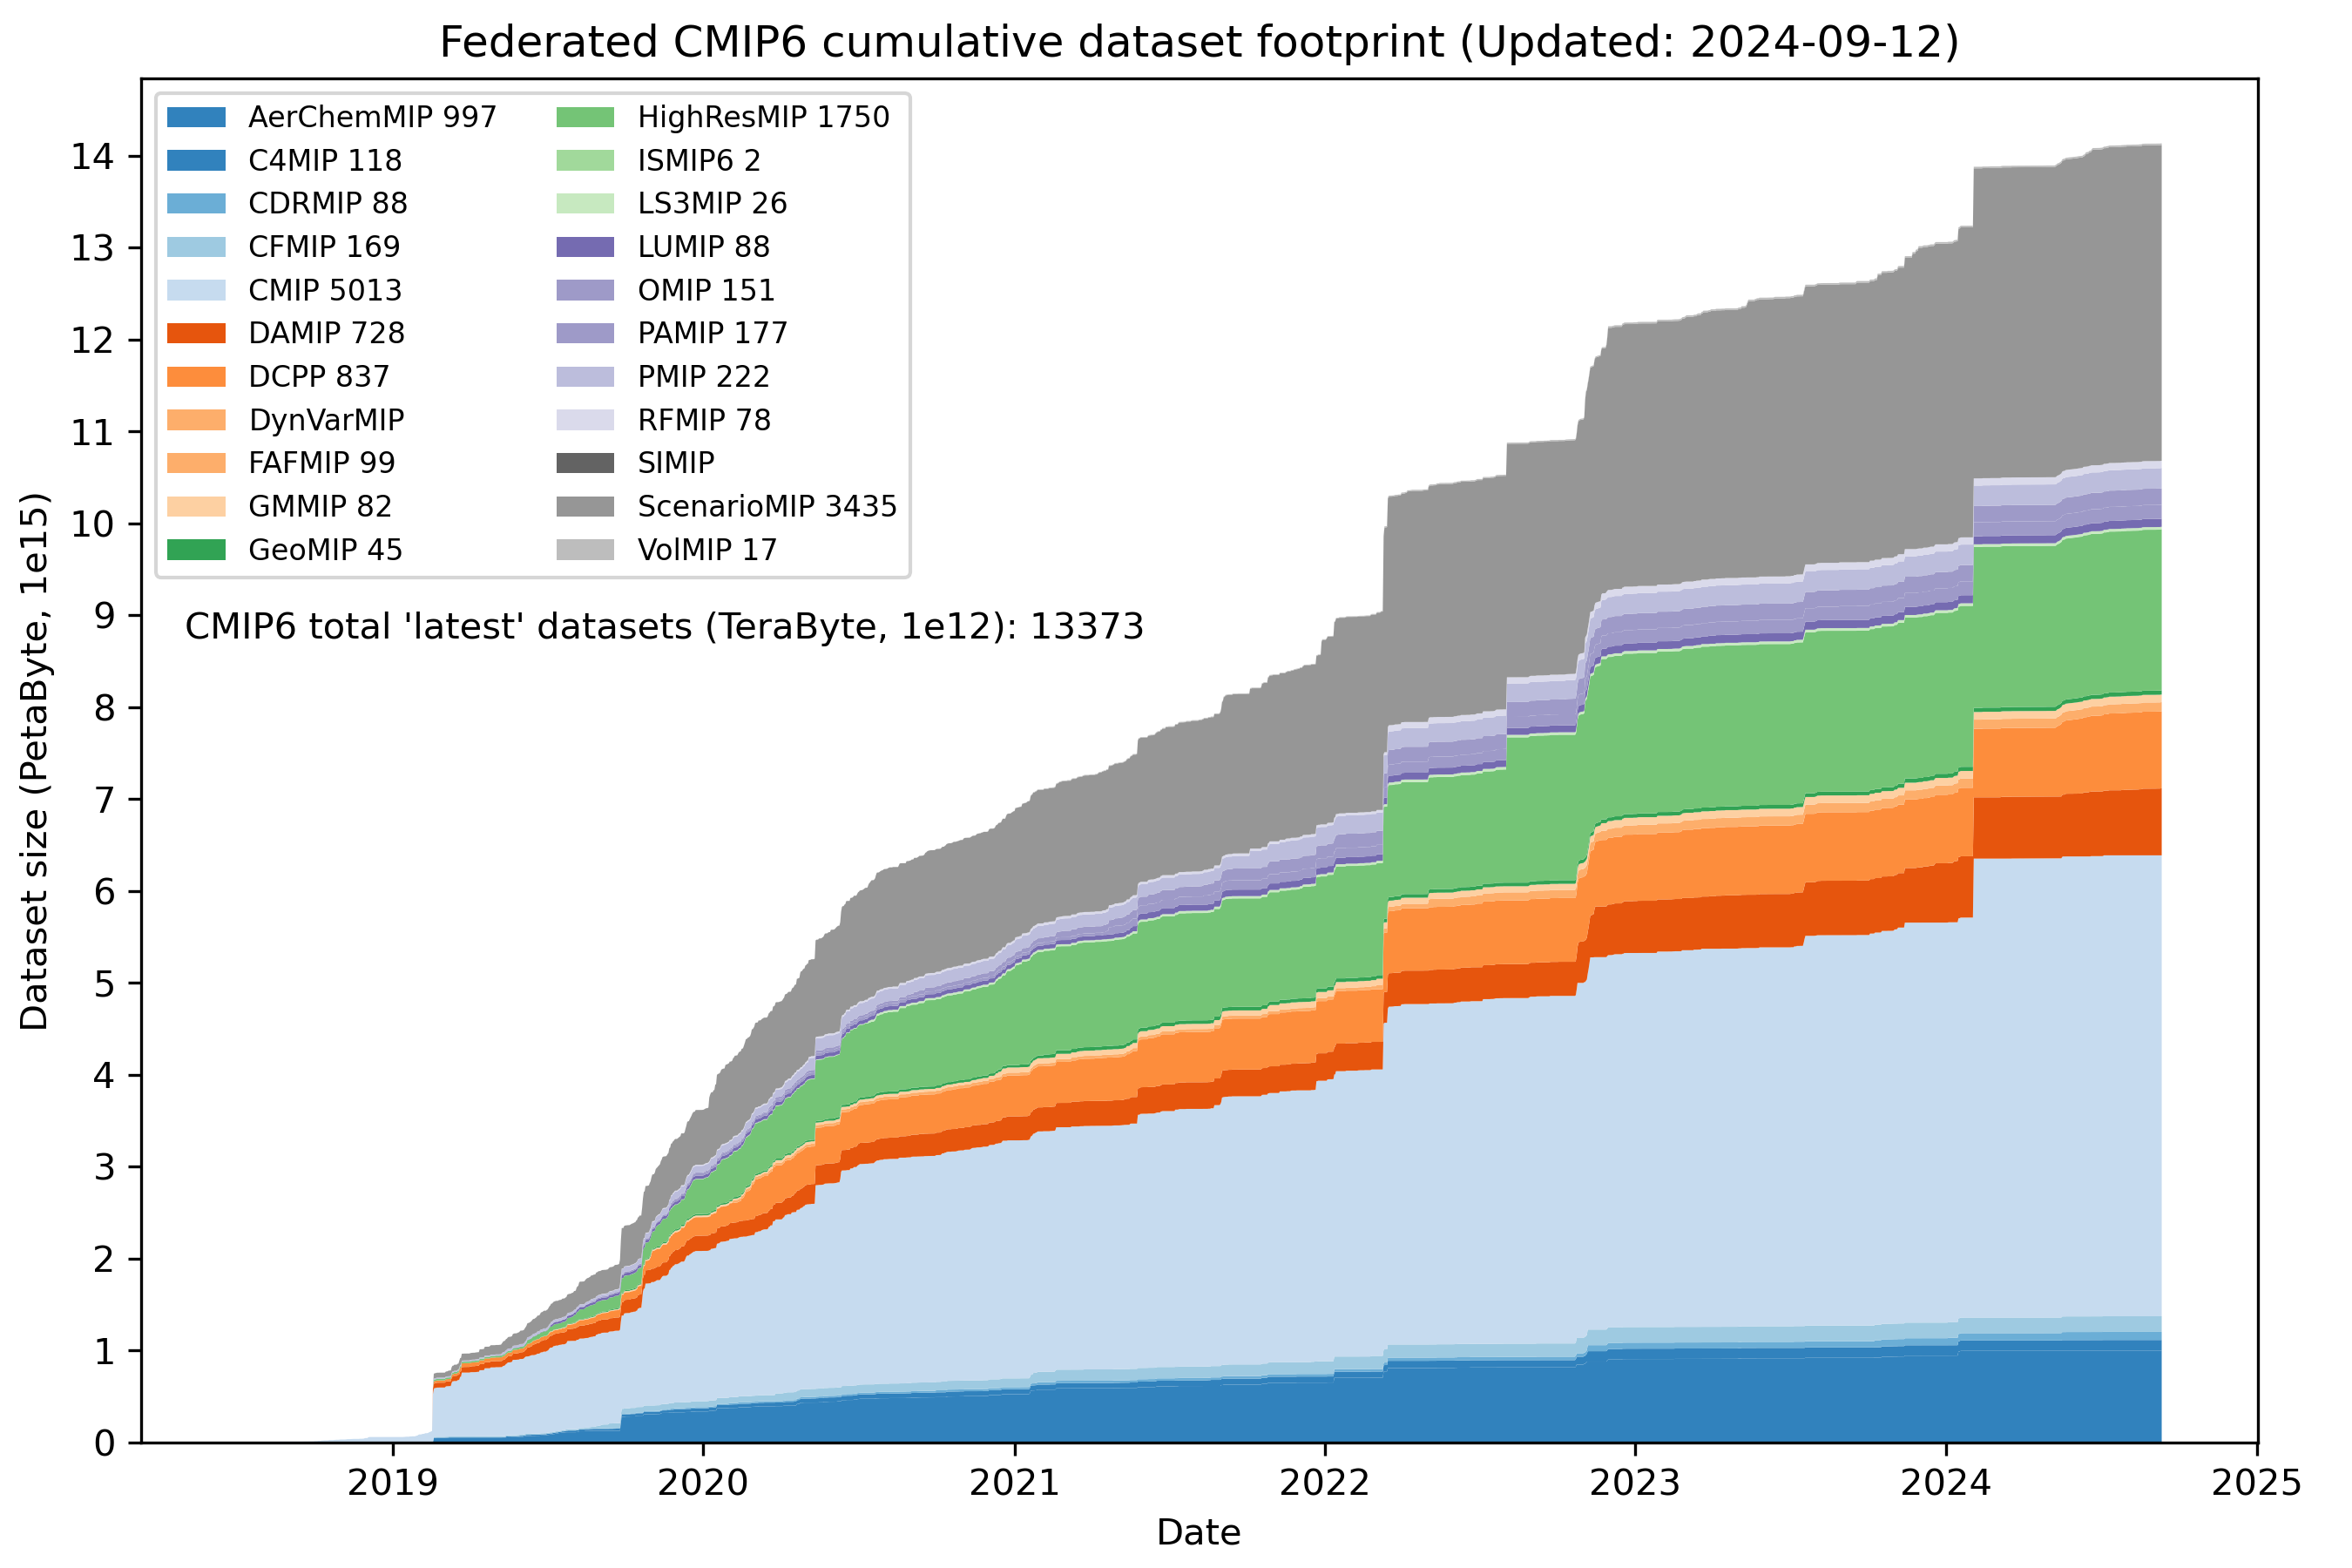
\includegraphics[width=1\linewidth]{240912T141943_ESGF-PublicationStatsPB.png}
    \caption{Growth of the CMIP6 project over time, with data sizes (PB) identified by colours for each of the CMIP6 Community MIPs (see \autoref{tab:tab2-CMIP6MIPs}) from the initial date of data publication (9th May 2018) through to the latest publication (September 2024). The largest data contributions in CMIP6 are from the CMIP (light blue) and ScenarioMIP (dark grey) activities, comprising 8.4 PB of the >15 PB total. Data growth fluctuated throughout the project's life, with current 2024 publication rates of 2.1 PB/yr (prorated). This compares to previous years: 0.8 in 2023, 3.3 in 2022, 1.8 in 2021, 3.1 in 2020, 3.3 in 2019, and 0.1 PB in 2018.}
    \label{fig:fig2-CMIP6DataGrowth}
\end{figure}


\subsection{The Earth System Grid Federation (ESGF)}
\label{sec:earthSystemGridFederation}

While addressing current climate science questions through coordinated experimentation is CMIP's core focus, facilitating data access and use by an exponentially growing international community has become a central project priority. 

As scientific momentum and ambitions grew through AMIP1/2, and early CMIP phases, like the early AMIP1 data, project data were collated on PCMDI hardware and, in many instances, shipped on hard drives from the modelling centre computing facilities. During AMIP's evolution, the dual remit of PCMDI led to the co-development of data formats and software packages targeting gridded climate data and storing and visualizing these growing archives. Consequently, in the early phases, much of the contributed data was rewritten into the PCMDI "standard" DRS (Data Retrieval and Storage) format, a netCDF file format precursor, and these data were made available to AMIP subproject registrants through a PCMDI file transfer protocol (FTP) server (\autoref{tab:tab1-MIPsThroughTime}; \citet{gates_amip_1995}).

By 2000, there was a US recognition that connecting parallel climate science activities across institutes and infrastructure made sense, broadening from the PCMDI single-site archive. By this stage, in addition to CMIP international efforts, parallel activities were underway at the National Center for Atmospheric Research (NCAR, USA) with the Community Climate System Model (CCSM), in addition to the Carbon-Land Model Intercomparison Project (C-LAMP) hosted at Oak Ridge National Laboratory (ORNL, USA) and copies of these data at the NERSC system that was housed at the Lawrence Berkeley National Laboratory (LBNL, USA). The ongoing collaborative work developing the federated US infrastructure was prototyped as the "Earth System Grid" (ESG I; \citet{bernholdt_earth_2007}) supported by DOE, which quickly gathered momentum with additional support from the DOE Scientific Discovery through Advanced Computing (SciDAC) program in 2002 in a second ESG II phase \citep{williams_earth_2009}. By late 2004, ESG II began distributing the CMIP3 data being collated in preparation for the IPCC Fourth Assessment Report (AR4). By the conclusion of CMIP3 in 2009, the 39 terabyte archive of model data had accumulated an order of magnitude more downloads (420 terabytes; \citet{ananthakrishnan_building_2007, williams_earth_2009}). Throughout the project lifetime, the hardware hosting the CMIP3 archive had failures, and there was a recognition that the centralized dependence on a single operational system wasn't sustainable long-term, particularly with the parallel growing demand to access and download these data.

By 2006, planning for the IPCC Fifth Assessment Report (AR5) was underway, and with it, CMIP5 (\autoref{sec:cmip5ProjectDesign}). The previous ESG successes led to the development of the next generation Earth System Grid Center For Enabling Technologies (ESG-CET), which included an expansion of collaborating institutions including Argonne National Laboratory (ANL, USA), Los Alamos National Laboratory (LANL, USA), National Oceanographic and Atmospheric Administration Pacific Marine Environmental Laboratory (NOAA-PMEL, USA) and the University of Southern California Information Sciences Institute (USA) \citep{ananthakrishnan_building_2007}, supported by the US DOE Offices of Advanced Scientific Computing Research (ASCR) and Biological and Environmental Research (OBER).

By 2008, infrastructure planning for CMIP5 had commenced, and a recognition was building that connecting international activities to augment the US-centric ESG-CET was needed \citep{williams_global_2016}. An agreement was signed in December 2008 between PCMDI, the British Atmospheric Data Centre (BADC, UK), and the World Data Centre for Climate, German Climate Computing Centre (DKRZ, Germany), identifying the Earth System Grid Federation (ESGF). These two European centres were leads of the IPCC Data Distribution Centre (IPCC-DDC), collating and archiving the climate model data used in preparing previous IPCC Assessment Reports. The ESGF goal was to develop a distributed federated architecture that would enable the compute storage resources at each of the centres to facilitate regional modelling groups to publish their CMIP5 model data to one of three nodes and then enable replication of these data across the federation, allowing the users to download or access CMIP5 data from their closest ESGF node \citep{williams_earth_2011}. In addition to the three core centres, additional ESGF nodes were established at the National Computational Infrastructure (NCI, Australia), National Aeronautics and Space Administration Jet Propulsion Laboratory (NASA-JPL, USA), NERSC (LBNL, USA), ORNL, and NCAR. At the CMIP5 peak, the ESGF had 50 \cred{\textbf{(CLARIFY NUMBERS, Karl?)}} active nodes hosting data and software \citep{williams_global_2016}.
\mycomment{
CMIP6 current nodes - https://aims2.llnl.gov/nodes
Very early CMIP5 http://web.archive.org/web/20111015000202/http://pcmdi3.llnl.gov/esgcet/home.htm 7 nodes ESG-CET + BADC, WDCC, NCI
ESG-CET NCAR, LLNL, ORNL https://extranet.gfdl.noaa.gov/~vb/curator/AR5-20071017/ESG-CET200710.pdf Oct 2007
2013 Aspen workshop - https://www.wcrp-climate.org/images/modelling/WGCM/WGCM17/WGCM17_report.pdf;
Middleton, Foster and Williams et al., 2006: Earth System Grid II final report 2001-2006 SCIDAC https://www.osti.gov/servlets/purl/1113798 https://doi.org/10.2172/1113798
}
\cred{Karl? The ESGF success in delivering CMIP5 led to the CMIP6 planning that began in 2013.. WGCM17}


\subsection{The IPCC Data Distribution Centre (IPCC-DDC)}
\label{sec:IPCC-DDC}
\cred{Attention Martina}


\subsection{Climate and Forecast (CF) Metadata conventions}
\label{sec:CFConventions}

By the early 1990s, the large (by the day's standards) climate model data archives had developed a considerable scientific following. With the augmented attention came the need to more clearly define model output quantities, their digital formats to ease data transfers and use, and documentation of the model configurations from where these data were derived. In parallel, there was considerable computer science development focused on generating a digital format that met the needs of growing meteorological data streams, with an aspiration to develop a portable and self-describing (where data and metadata that described it were co-contained) file format that allowed relevant metadata to be embedded alongside the data matrices. These discussions occurred parallel to the early MIP phases but led to numerous early releases of the network Common Data Format (netCDF) through the late 1980s and early 1990s. In May 1997, netCDF 3.3 was released, which included a new type-safe interface for the C and Fortran languages. In March 2001, netCDF 3.5.0 was released, which integrated a new Fortran90 interface, making this library suitable for integration with climate model libraries primarily written in Fortran \cred{(REFs?)}.
\mycomment{
https://docs.unidata.ucar.edu/nug/2.0-draft/netcdf_history.html
}

In parallel to the netCDF digital format and language interface development, the ability to store rich self-describing metadata within the file led to considerable work on data conventions. Of climate data relevance, the first was developed by the Cooperative Ocean/Atmosphere Research Data Service (COARDS), a NOAA and US university cooperative aimed at sharing and distributing global atmospheric and oceanographic research datasets. COARDS 1.0 was released in February 1995 and laid out data variable conventions such as assigning spatial dimension/coordinate attributes (height, latitude, longitude) and data variable attributes (long\_name, missing\_value, units), in addition to some required global attributes (e.g., title) providing descriptive context for the data. Much of the COARDS work aided the Ferret visualization and analysis environment development, with Ferret 4.0 released in March 1995 \cred{(REFs?)}. This data standardisation aided the coordination of software efforts, reducing parallel package development into a couple of well-supported packages targeting the evolving COARDS conventions.
\mycomment{
https://ferret.pmel.noaa.gov/Ferret/documentation/coards-netcdf-conventions
https://ferret.pmel.noaa.gov/static/Documentation/Release_Notes/v400.html
Also NCAR CSM - see http://cfconventions.org/conventions.html
}

By 1997, the large and growing MIP archives had accumulated tens of thousands of output files from tens of model configurations. There was a need to enforce standardization on model outputs to aid their ease of use by a diverse and growing international community. The Gregory, Drach, and Tett (GDT v0; \citet{gregory_gdt_1999}) standards were first released in June 1997 to fill this void. The GDT standard expanded markedly on COARDS, with a prime focus on better defining GCM output to be self-describing and conform to standard conventions that detailed longitude, latitude, height/depth, coordinate/grid bounds, time, calendars and climatologies, missing values, and data compression. In 1999, the continued development of GDT ceased at v1.4, with the effort led by Unidata (USA) to amalgamate parallel efforts into what became known as the NetCDF Climate and Forecast (CF) Metadata Conventions. The CF Conventions v1.0 was first released in October 2003 having expanded markedly on the COARDS, GDT and numerous other parallel efforts that preceded it.

\cred{Karl? This could be markedly augmented with your first-hand knowledge. With the evolution from CF early days to v1.11 and the grid specifications being folded in}

\mycomment{
https://www.unidata.ucar.edu/software/netcdf/conventions.html
https://www.unidata.ucar.edu/software/netcdf/coords/proposals.html
COARDS 1995 - https://web.archive.org/web/20100527095818/http://ferret.wrc.noaa.gov/noaa_coop/coop_cdf_profile.html
GDT 1997
https://www.unidata.ucar.edu/mailing_lists/archives/netcdfgroup/1997/msg00080.html
https://www.unidata.ucar.edu/software/netcdf/coords/0054.html 1997
https://web.archive.org/web/20100610102527/http://www-pcmdi.llnl.gov/drach/GDT_convention.html 1999
https://web.archive.org/web/20040604041414/http://www-pcmdi.llnl.gov/drach/netCDF.html
CF 2003 - https://cfconventions.org/Data/cf-conventions/cf-conventions-1.11/cf-conventions.html#_version_1_0_28_october_2003 
}


\subsection{Controlled vocabularies (CVs)}
\label{sec:CMIPCVs}
\cred{Attention Karl, Paul Need to consider realm evolution across mip eras, which dovetails the Variable request etc following section}

The experiences coordinating large and growing international climate science activities through AMIP1/2 and the early CMIP phases, coupled with parallel infrastructure and convention development, allowed for a common nomenclature to evolve defining and describing the various model outputs.

By CMIP3, 16 modelling groups were consistent participants, contributing to the preceding AMIP1/2, CMIP1, and CMIP2/2+ phases (\autoref{fig:fig1-MIPGrowth}). The regular contributions from known modelling groups (institutions), in many instances with known model names (many identified with a numeric version) allowed for acronyms to be created providing continuity across the model versions and phases. In addition, the more coordinated experimental protocols, now numbering 12 (see \autoref{tab:tab1-MIPsThroughTime}), and the identification of these activities as collections of MIPs (e.g., AMIP, CMIP, CFMIP, PMIP) also allowed experiment acronyms to be created which through NetCDF conventions, allowed for unique identities, filenames, and metadata to be defined. For CMIP3, development of the CMOR1 software \citep{taylor_cmor_2006} along with the CMIP3-CMOR-Tables \citep{doutriaux_cmip3_2005}, organized the 362 variables requested (see \autoref{tab:tab1-MIPsThroughTime}), greatly facilitated the standardization of file metadata that is now common, allowing CMIP3 documentation requirements to be specified (\citet{taylor_pcmdi_2005}). For the first time, this enabled modelling groups to describe their data following the guidance and for this data to be organized on the PCMDI computing systems by contributing model, experiment, variable, and CMOR table \citep{doutriaux_cmip3_2005} which considerably aided the automated replication and organization of the archive.

This process continued in CMIP5, with an increase to 26 modelling groups and an expansion in sub-MIPs leading to 34 experiments making up the phase (\autoref{tab:tab1-MIPsThroughTime}, \autoref{fig:fig1-MIPGrowth}).  For CMIP5, the CMOR2 software was developed \citep{doutriaux_cmor_2011} along with the CMIP5-CMOR-Tables \citep{doutriaux_cmip5_2013} which captured a dramatic increase in the variables requested, now totalling 1026 (see \autoref{tab:tab1-MIPsThroughTime}). CMOR2 expanded the standardized metadata that was written to output files, building on the improvements in CMIP3 \citep{taylor_pcmdi_2010}, and in addition imposed standard filenames and directory structures \citep{taylor_pcmdi_2012}, which further aided unique data identities and was necessary to facilitate the growing archives across the now federated ESGF data distribution infrastructure (see \autoref{sec:earthSystemGridFederation}). This phase also incorporated dataset version information, assigned during the data preparation and ESGF publication process, allowing for errors to be identified and associated with a data version, greatly aiding more systematic replication and dataset status identity. 

For CMIP6 this evolution continued, with the development of CMOR3 \citep{mauzey_cmor_2024}. The dramatic project expansion with federated sub-MIPs led to a ballooning project, increasing to include 49 contributing modelling groups and 322 experiments (\autoref{tab:tab1-MIPsThroughTime}). Due to the broadening of model diversity and configurations used across this large experimental expansion, a dedicated data request was needed, tying variables requested by MIP/experiment (see \autoref{sec:CMIP6DR}). In total, 2062 variables were requested across all experiments, encoded into the CMIP6-CMOR-Tables \citep{nadeau_cmip6_2017}. Like the phases before it, this led to a further expansion of identifiers and metadata \citep{taylor_pcmdi_2018}, aiding unique data identities and the routine replication of data across the now large international ESGF federation.

\mycomment{
For CMIP6, as work on numerous parts of the infrastructure began, their collation of CMIP6 project information occurred independently from one another (ES-Docs, CMIP6 Data Request, and WIP CVs). There was agreement at a WIP meeting in June 2016 (here) that core CMIP6 information needed to be centralized in a single authoritative format for all downstream infrastructure to use, which by that time included the CMIP6 Data Request, ES-Docs, DKRZ Citation Service, ESGF and the modelling-group-serving CMOR and cmip6-cmor-tables. In November 2016 the first instance of the centralized CVs was initiated by the WIP developed as the CMIP6_CVs - https://github.com/WCRP-CMIP/CMIP6_CVs. Previous to this, the CMIP6 Data Request (Martin), ES-Docs (Eric Guilyardi and team) and the WIP (Balaji and Karl) had been collating information from the CMIP Panel and MIP Chairs directly. There had been no direct information collation from modelling groups, however, discussions with the CMIP Panel Chair had been ongoing. Once there was a WIP agreement to centralize this information, the activity_id’s, experiment_id’s, institution_id’s and source_id’s were defined (see initial release here), which became the centralized and managed source of information about the CMIP6 project phase, and began the process of harmonizing activity_id/MIP and experiment_id’s across the infrastructure. This also allowed the late registration of new MIPs (CDRMIP and PAMIP in April 2018) and amendments and augmentations to existing MIP experiments, to weed out duplication and more tightly refine the experiment list.
In parallel Martin was working on the CMIP6 Data Request, which began from the information contained in the cmip5-cmor-tables (with familiar table names, e.g., CMIP5_Amon), and built up the CMIP6 variable list which ~doubled over eras (CMIP5 ~970 to CMIP6 2062). To enable modelling groups to encode their simulation data into the CMIP6 format, CMOR3 was developed with the first 3.0-alpha released on 1 Feb 2016, which required the cmip6-cmor-tables to be defined before this was usable. The cmip6-cmor-tables were first released in June 2017 (here) aligning with version 01.00.11 of the CMIP6 Data Request, with work starting on the CMIP6 Data Request translation in January 2016 (here).
For CMIP6Plus (in preparation for CMIP7) the planning has been to address issues raised with the CMIP6 infrastructure (a high-level overview of the issues are outlined in the CMIP6Plus whitepaper here. Numerous other feedback has been collected over the past years, with some more complete than others, e.g., feedback from CERFACS, CNRM and IPSL here). We have recognized repeating issues over CMIP phases that are far better addressed in a modular way. After broad consultation, the approach that is being prototyped through CMIP6Plus_CVs (https://github.com/WCRP-CMIP/CMIP6Plus_CVs) is now in place. The CVs Drop-in, held online on the 8 November 2023 summarised the plans and progress (slides here, other materials here, drop-in report here, recording ?here?). It was an open opportunity for feedback across everyone interested in contributing. Indeed both GitHub repositories are open access, with anyone with a GitHub account able to clone the repo, create issues or submit a pull request with content.
}


\subsection{Variable request and standard output}
\label{sec:CMIP6DR}
\cred{Attention Karl, Peter G and Martin J}
\cred{Need to consider realm and frequency evolution across mip eras, what else? RE: realm evolution, started in CMIP3 with tables (A1, O1, etc), built around the history files, built around model components - so all ocean history files contained ocean, and sea ice variable, etc - Karl to augment; RE: frequencies, 3D fields, vs 2D fields were separated across tables as these had different temporal requests, to keep request sizes down}
\autoref{tab:tabAppB1-MIPStandardOutput}

{\color{blue} For any simulation, models produce fields of climate- and weather-relevant information covering temporal scales from minutes to centuries. Not all information of conceivable interest can be archived due to resource constraints both in terms of post-processing effort and in terms of available storage. Experiment planners must anticipate how essential each model-produced field will be for achieving its objectives and decide whether the fields should be reported at monthly, daily, or sub-daily time-intervals. The challenge is to limit the "standard output" requested from a model experiment to the minimum required, and then request, at lower priority, other variables of interest, which are not critical to achieving the primary objectives.}

\sout{A critical component MIP experimentation is specifying what simulation output to save. It is a trade off between the efforts required by modelling groups to fulfill a request, available storage, and existing and potential future science needs. Despite advancing technology, saving everything (i.e., all prognostic variables at every timestep) has never been realistic. In AMIP1/2, CMIP1/2/2+/3/5, consideration, was made in consultation with MIP chairs and modelling groups about what questions or analyses will be pursued with a given simulation that dictates how much data is saved.} 

{\color{blue}In the pre-MIP era, the FANGIO experiments were focused almost entirely on a single objective: to determine whether clouds were responsible for the range of global climate sensitivities found in models. The narrow objective meant that the required output was limited to a few fields and, primarily, the global mean of those fields.}  

{\color{blue}When AMIP was proposed, the potential scope of objectives expanded considerably, spanning both time-scales and spatial scales.} \sout{As MIPs emerged, more scientists began analyzing simulations, and it was not always clear a priori what would be studied.} The most basic or routine climate model output {\color{blue} was} \sout{is} arguably monthly means, \sout{so one question often is which variables to save. However,} {\color{blue}but} even in the early days of AMIP1, scientists were interested in process-level analyses to understand model responses\sout{ more deeply}, which required daily or even higher temporal frequency fields.

In AMIP1, {\color{blue}storage and resource limitations were a primary concern in defining the standard output list. The requested output was agreed following extended discussion and negotiation involving} \sout{boundaries were pushed based on the amount of saved data. To define the standard output list, discussions between} the WCRP WGNE \sout{panel}, PCMDI, contributing modellers, and other {\color{blue}tightly-engaged} scientists \sout{who were closely engaged in the process that defined the request}. Enough temporal mean data was saved to {\color{blue}serve the numerous subprojects that were subsequently established to systematically evaluate in novel ways a diversity of model characteristics} \sout{enable many scientists to complete their diagnostic subprojects} \citep{gates_amip_1995}. \sout{evaluating a diversity of model characteristics in ways that had never been done before. But it was not enough, and only the beginning. For AMIP2, continued discussions focused on more in-depth scientific investigations and advanced a more comprehensive set of AMIP standard output.} 

{\color{blue}Seeing the interest in AMIP grow, modeling groups began to realize that there could be benefits of providing an expanded set of model output because it would enable a wider range of analyses and possibly lead to new insights about model behavior. Thus, in AMIP2 the standard output more than tripled (from 32 to 114) and for the first time included 6-hourly data, which was particularly useful in studying weather phenomena} \sout{For the first time, this included 6-hourly data, in addition to the monthly mean data requested in AMIP1 }(\autoref{tab:tab1-MIPsThroughTime}), \sout{expanding the variables from 32 to 114} (see \autoref{tab:tab1-MIPsThroughTime}). In addition, {\color{blue} the} monthly mean\sout{s of selected} covariances \sout{that} needed to \sout{be computed on the fly were added, offering the possibility of evaluating the} {\color{blue}evaluate a model's} Lorenz energy cycle {\color{blue} were reported. These co} \sout{as simulated by the models. Co-}variances {\color{blue} did in fact enable the intended analysis} \sout{facilitated some interesting work} \citep{boer_energy_2008}, {\color{blue}but modeling groups felt that given their limited use, the effort required in computing them was unwarranted}. \sout{Still, it was also a lesson in the delicate balance of what output to save because they are computationally expensive products for modelers to provide.} Since AMIP2, co-variances have not been part of the routine output request and have only been saved for targeted studies.

{\color{blue}Compared with AMIP2, CMIP1's standard output list was modest, }\sout{The CMIP1 standard output began very conservatively when contrasted to AMIP2,} with just 23 variables requested (\autoref{tab:tab1-MIPsThroughTime}).  {\color{blue} The CMIP1 experiment was a control run with a focus on mean climatology, so most variables requested were summer and winter mean fields, but there were also} \sout{representing a handful of time average and} three multi-year monthly mean surface fields requested. Like AMIP, what to save was defined by scientists directly involved in advancing the project, including the WGCM and PCMDI. Also like AMIP, the initial standard output list would inevitably grow over subsequent phases, as its scientific impact became apparent. \sout{data was only a stepping stone of what was to come.}  

\sout{For CMIP3, there was a somewhat more concerted effort to define the model output, but it was still done within a small community that was open to feedback from interested scientists but had to balance the practical limits of the data volume with the potential benefits. <Should the infamous Taylor spreadsheets be pointed to? KET: I don't think the spreadsheets came along until CMIP5>.}

{\color{blue}Although CMIP2 saw only a small increase in CMIP's scope, in CMIP3 both the number of experiments and the standard output requested increased by an order of magnitude.  CMIP output was expected to serve an increasingly wide diversity of scientific analyses, and the historical and future scenario runs would begin serving those studying climate impacts. For such purposes, the variables of most interest to those developing models were augmented with variables characterizing changes near the surface and climate "extreme indices" that might be used to assess impacts.  Like the AMIP2 covariance statistics, the extreme indices were difficult to compute and subsequently were eliminated from future lists of standard output.  This is another example of how the CMIP standard model output has in some cases been culled for practical reasons.

As in earlier phases, the CMIP Panel and PCMDI coordinated the effort to define the CMIP3 output, but input was sought from those with specialized scientific expertise in areas such as clouds (e.g., regarding the ISCPP simulator input needed by those involved in the  Cloud Forcing Model Intercomparison Project) or impacts (e.g., regarding the extreme indices).

CMIP5 represented a second step change in the size and complexity of the standard output request. The number of experiments tripled to 34 (or 36???) and the number of number of different variables tripled to just over 1000. For the first time, CMIP attempted to coordinate the experiments designed by multiple, independent MIPs.  As before, a common set of standards was imposed on model output.  A single comprehensive list of variables was compiled and organized into 13 tables. For each experiment defined by a MIP, variables were requested by table; all the variables in a requested table were to be reported, but sometimes only for a portion of a simulation. Each table contained variables produced (usually) by a single model component (e.g., atmosphere, ocean, sea ice, land) and reported at a single frequency (e.g., 3-hourly, daily, monthly).  CFMIP required special variables that were not needed by most other MIP experiments.  To meet their needs, an additional 5 tables (divided into 10 sub-tables) were defined.  All tables of variables were accessible as spreadsheets or as machine-readable text files.  The mapping of experiments to the tables/variables that were requested could only be done by reading the spreadsheet and was not well-suited for automation.  }



\cred{KARL, I think you can fill in the blanks better than I here...}

With more experiments and more scientists with varied interests involved, the process transformed from being defined by a limited group of scientists involved in the MIPs as standard experiment output to "Data Request."

Alongside the vast expansion in MIP activity through the 1990s and 2000s (\autoref{sec:cmip6InContext}), the concept of climate model "standard output" had been a building feature of the progressive MIP phases.

\cred{this would be a useful point to contrast the requested/2062 variables vs the realized}

\mycomment{
The CMIP6 "data request" \citep{juckes_cmip6_2020} was the most comprehensively outlined preceded by three decades of evolution in climate model understanding. This history underpinned the development of the standard experimental protocols 
\citet{gates_amip_1991} - AMIP1
\citet{gates_amip_1993} - AMIP History Archive
\citet{gates_amip_1994} - AMIP Ensemble
\citet{gleckler_amip_1996} - AMIP 7 monthly mean and six-hourly output, plus ensembles/AMIP 2
\citet{gleckler_amip_1996-1} - AMIP number 8, STANDARD OUTPUT low and high frequency (6-hr)
https://pcmdi.llnl.gov/mips/amip/OUTPUT/WGNEDIAGS/index.html
\citet{taylor_pcmdi_2009}
\citet{taylor_pcmdi_2013}
\citet{juckes_baseline_2024}

FANGIO not multi-year (perpetual July)/January; AMIP1 success, multi-year SST/sea-ice (Russians and Chinese); AMIP2 next-level output, more high frequency data, mean products (covariances; u/v-prime overbar - on the fly calculation) monthly mean timeseries (Boer \& Lambert 2008, clim dyn - relationship to Lorenz energy cycle)
CMIP2: https://pcmdi.llnl.gov/mips/cmip2/
CMIP3: https://pcmdi.llnl.gov/mips/cmip3/experiment.html
CMIP5: https://pcmdi.llnl.gov/mips/cmip5/requirements.html
}
\cred{\textbf{Figure which captures the requested and realized/published data across CMIP3, CMIP5, CMIP6 - this can be lifted from the *-cmor-tables and the ESGF indexes directly}}


\subsection{Model (and data) documentation}
\cred{Attention Bryan Lawrence, David Hassell; David H noted of the WIP telco 241022 that CMIP5/Metafor \citep{guilyardi_cmip5_2011} was overly constrained [drop down boxes], CMIP6/ES-Docs \citep{pascoe_documenting_2020} was too loosely constrained, and with the CMIP7 EMD this should hopefully hit the sweet spot}


\subsection{Data citation}
\cred{Attention Martina}
With exponential growth in both the climate community using data, and CMIP archive of model output over phases (\autoref{tab:tab1-MIPsThroughTime}), the need to more explicitly assign credit to modelling groups, in addition to uniquely identifying model data used for downstream analyses, tracking errata, and enabling reproducible science, was needed. Before the distributed and federated ESGF development (\autoref{sec:earthSystemGridFederation}), a single location PCMDI hosted the complete AMIP and CMIP archives, but this changed in CMIP5. For this phase, three primary nodes at PCMDI (California, USA), The German Climate Computing Centre (DKRZ, Hamburg, Germany) and Centre for Environmental Data Analysis (CEDA, Oxfordshire, UK), shared the hosting role for the CMIP5 archive - distributed across nodes and not complete at any one centre. Data federation led to a more complex task in keeping track of uniquely identifying datasets. To solve this problem, DKRZ led an effort to both quality control and assign Digital Object Identifiers (DOIs) to CMIP5 datasets \citep{stockhause_quality_2012, stockhause_cmip6_2017}, delivered alongside the long-term archival as part of the DKRZ IPCC Data Distribution Center (IPCC-DDC, \citet{stockhause_twenty-five_2022}).

Following CMIP5, for CMIP6, a more ambitious plan was established to meet the needs of IPCC-DDC archived data and the evolving data real-time \citep{stockhause_cmip6_2017}. Considering the CMIP project evolution across phases and the federated design that underpinned CMIP6 (\autoref{sec:cmip6ProjectDesign}, \citet{eyring_overview_2016}), data citation needed to account for model configurations that were targeted across the 23 MIPs that published data to the project (\autoref{tab:tab2-CMIP6MIPs}). To date, 2,693 CMIP6 DOIs have been generated, with the first issued to the first CMIP6 dataset published in May 2018 (see \autoref{fig:fig2-CMIP6DataGrowth}). CMIP6 DOIs provide two levels of citation support, one targeted at the upper level, a model (source\_id), and another at the lower experiment (experiment\_id) level, allowing a user to more tightly attribute the dataset used.

\cred{Some information about total citations, persistence, other information, other references?}
\mycomment{
https://www.wdc-climate.de/ui/statistics?type=cmip6_doi_registration
https://commons.datacite.org/repositories/8orcv25 - Master overview 6012 citations
https://www.wdc-climate.de/ords/f?p=127:2 - CMIP6 data references
https://www.wdc-climate.de/ui/cmip6?input=CMIP6.ScenarioMIP.NOAA-GFDL.GFDL-CM4.ssp585
https://www.wdc-climate.de/ui/cmip6?input=input4MIPs.CMIP6.CMIP.PCMDI
}


\subsection{Data errata}
\cred{Attention Guillaume L., Atef B.-N.}

The growing coherence across successive CMIP archives allowed for more complete data tracking and the development of an errata list documenting user-reported problems. For CMIP3 and CMIP5, user reports via email were captured by PCMDI, and the tabulated information was hosted on an external-facing website and reported to the relevant modelling centre. The process was slow, but did yield a collated error list representing issues across the archive, and which led to several data revisions fixing reported issues (see \autoref{tab:tabAppC1-MIPErrata}). For CMIP3, user-reported errors led to the retraction of all simulations from a single modelling centre, as a significant bug was found in the model formulation rendering its output obsolete.

\cred{For CMIP6, this process was considerably augmented.}


\subsection{Data downloads}
\cred{Attention Sandro Fiore
\begin{itemize}
	\item ESG download history and CMIP3 (LLNL/PCMDI)
    \item History of CMCC ESGF involvement
	\item CMIP5 statistics
	\item CMIP6 statistics
\end{itemize}
}

\section{CMIP6 supporting projects}
\label{sec:CMIP6SupportingProjects}
In addition to the core infrastructure that has delivered past CMIP phases, several supporting projects have been in development over the past decade. Below is a brief overview of these activities.



\subsection{input4MIPs: climate forcing}
\label{sec:input4MIPs}
\cred{Attention Paul}

Data

\cred{AMIP Forcing \citet{gleckler_amip_1996-1} - AMIP number 8, solar constant, CO2, ozone, land use; PCMDI IPCC 4AR simulations and forcing Curt/Karl;  \citet{durack_toward_2018}}
\mycomment{
CMIP3
https://pcmdi.llnl.gov/mips/cmip/ann_20c3m.html
https://web.archive.org/web/20040706074446/http://www-pcmdi.llnl.gov/cmip/
https://web.archive.org/web/20040827091054/http://www-pcmdi.llnl.gov/cmip/
CMIP5
https://pcmdi.llnl.gov/mips/cmip5/forcing.html
Old information CMIP paths
/Users/durack1/sync/Docs/admin/LLNL/12/120607_PaulDurack_PCMDI-CMIP5DataMeeting_LLNL.pdf
/Users/durack1/sync/Docs/admin/LLNL/17/151202_covey1_CMIP1And2/151202_covey1-CMIP1Documentation.pdf
/Users/durack1/sync/Docs/admin/LLNL/17/151202_covey1_CMIP1And2/170530_gleckler1_CMIPPaths.pdf
}


\subsection{obs4MIPs: observed data for model evaluation}
\cred{Attention Peter G; \citet{teixeira_satellite_2011}, \citet{waliser_observations_2020}}



\subsection{Coordinated evaluation}
\cred{need to place community evaluation in context with the A/CMIP subprojects, ala \citet{gates_amip_1992}}

Model evaluation and benchmarking are crucial in assessing climate models, helping to quantify their performance and identify areas for improvement. Over the years, several tools have been developed to streamline this process, particularly in the context of the CMIP (Hoffman et al., 2024 [in prep]). The PCMDI Metrics Package (PMP) is one of the key tools, providing a standardized framework for evaluating climate models by comparing their outputs with observations from obs4MIPs across a range of variables focusing on physical climate and their variabilities \citep{gleckler_more_2016,lee_systematic_2024}. ILAMB (International Land Model Benchmarking) focuses on assessing land surface models, offering comprehensive diagnostics and benchmarking to evaluate their representation of land-atmosphere interactions \citep{collier_international_2018}. Similarly, the ESMValTool (Earth System Model Evaluation Tool) supports the analysis and evaluation of Earth system models by incorporating a wide array of observational datasets and diagnostics, enabling multi-model comparisons \citep{eyring_overview_2016}. These and other tools available in the community as reviewed by Hoffman et al. (2024) play pivotal roles in ensuring that models participating in CMIP meet rigorous scientific standards, facilitating ongoing model improvement and fostering transparency in model evaluation. Together, they have significantly advanced the field of climate model assessment, contributing to the evolution of CMIP phases by providing quasi-operational evaluation capabilities, for example, as demonstrated in the past IPCC AR reports \citep{mcavaney_model_2001,flato_evaluation_2013,eyring_human_2021}.

To leverage these tools more efficiently and immediately, the WCRP established the Climate Model Benchmarking Task Team, which aims to provide a systematic and rapid performance assessment of CMIP models, particularly for the expected CMIP7 participating models. The Task Team proposed the concept for a new Rapid Evaluation Framework (Hoffman et al. 2024 [in prep]), whose development is initiated and in progress for CMIP AR7 Fast Track simulations to support the next IPCC Assessment Report 7 (AR7) cycle.


% all figures and data should live in standalone github repo
\begin{figure}
    \centering
    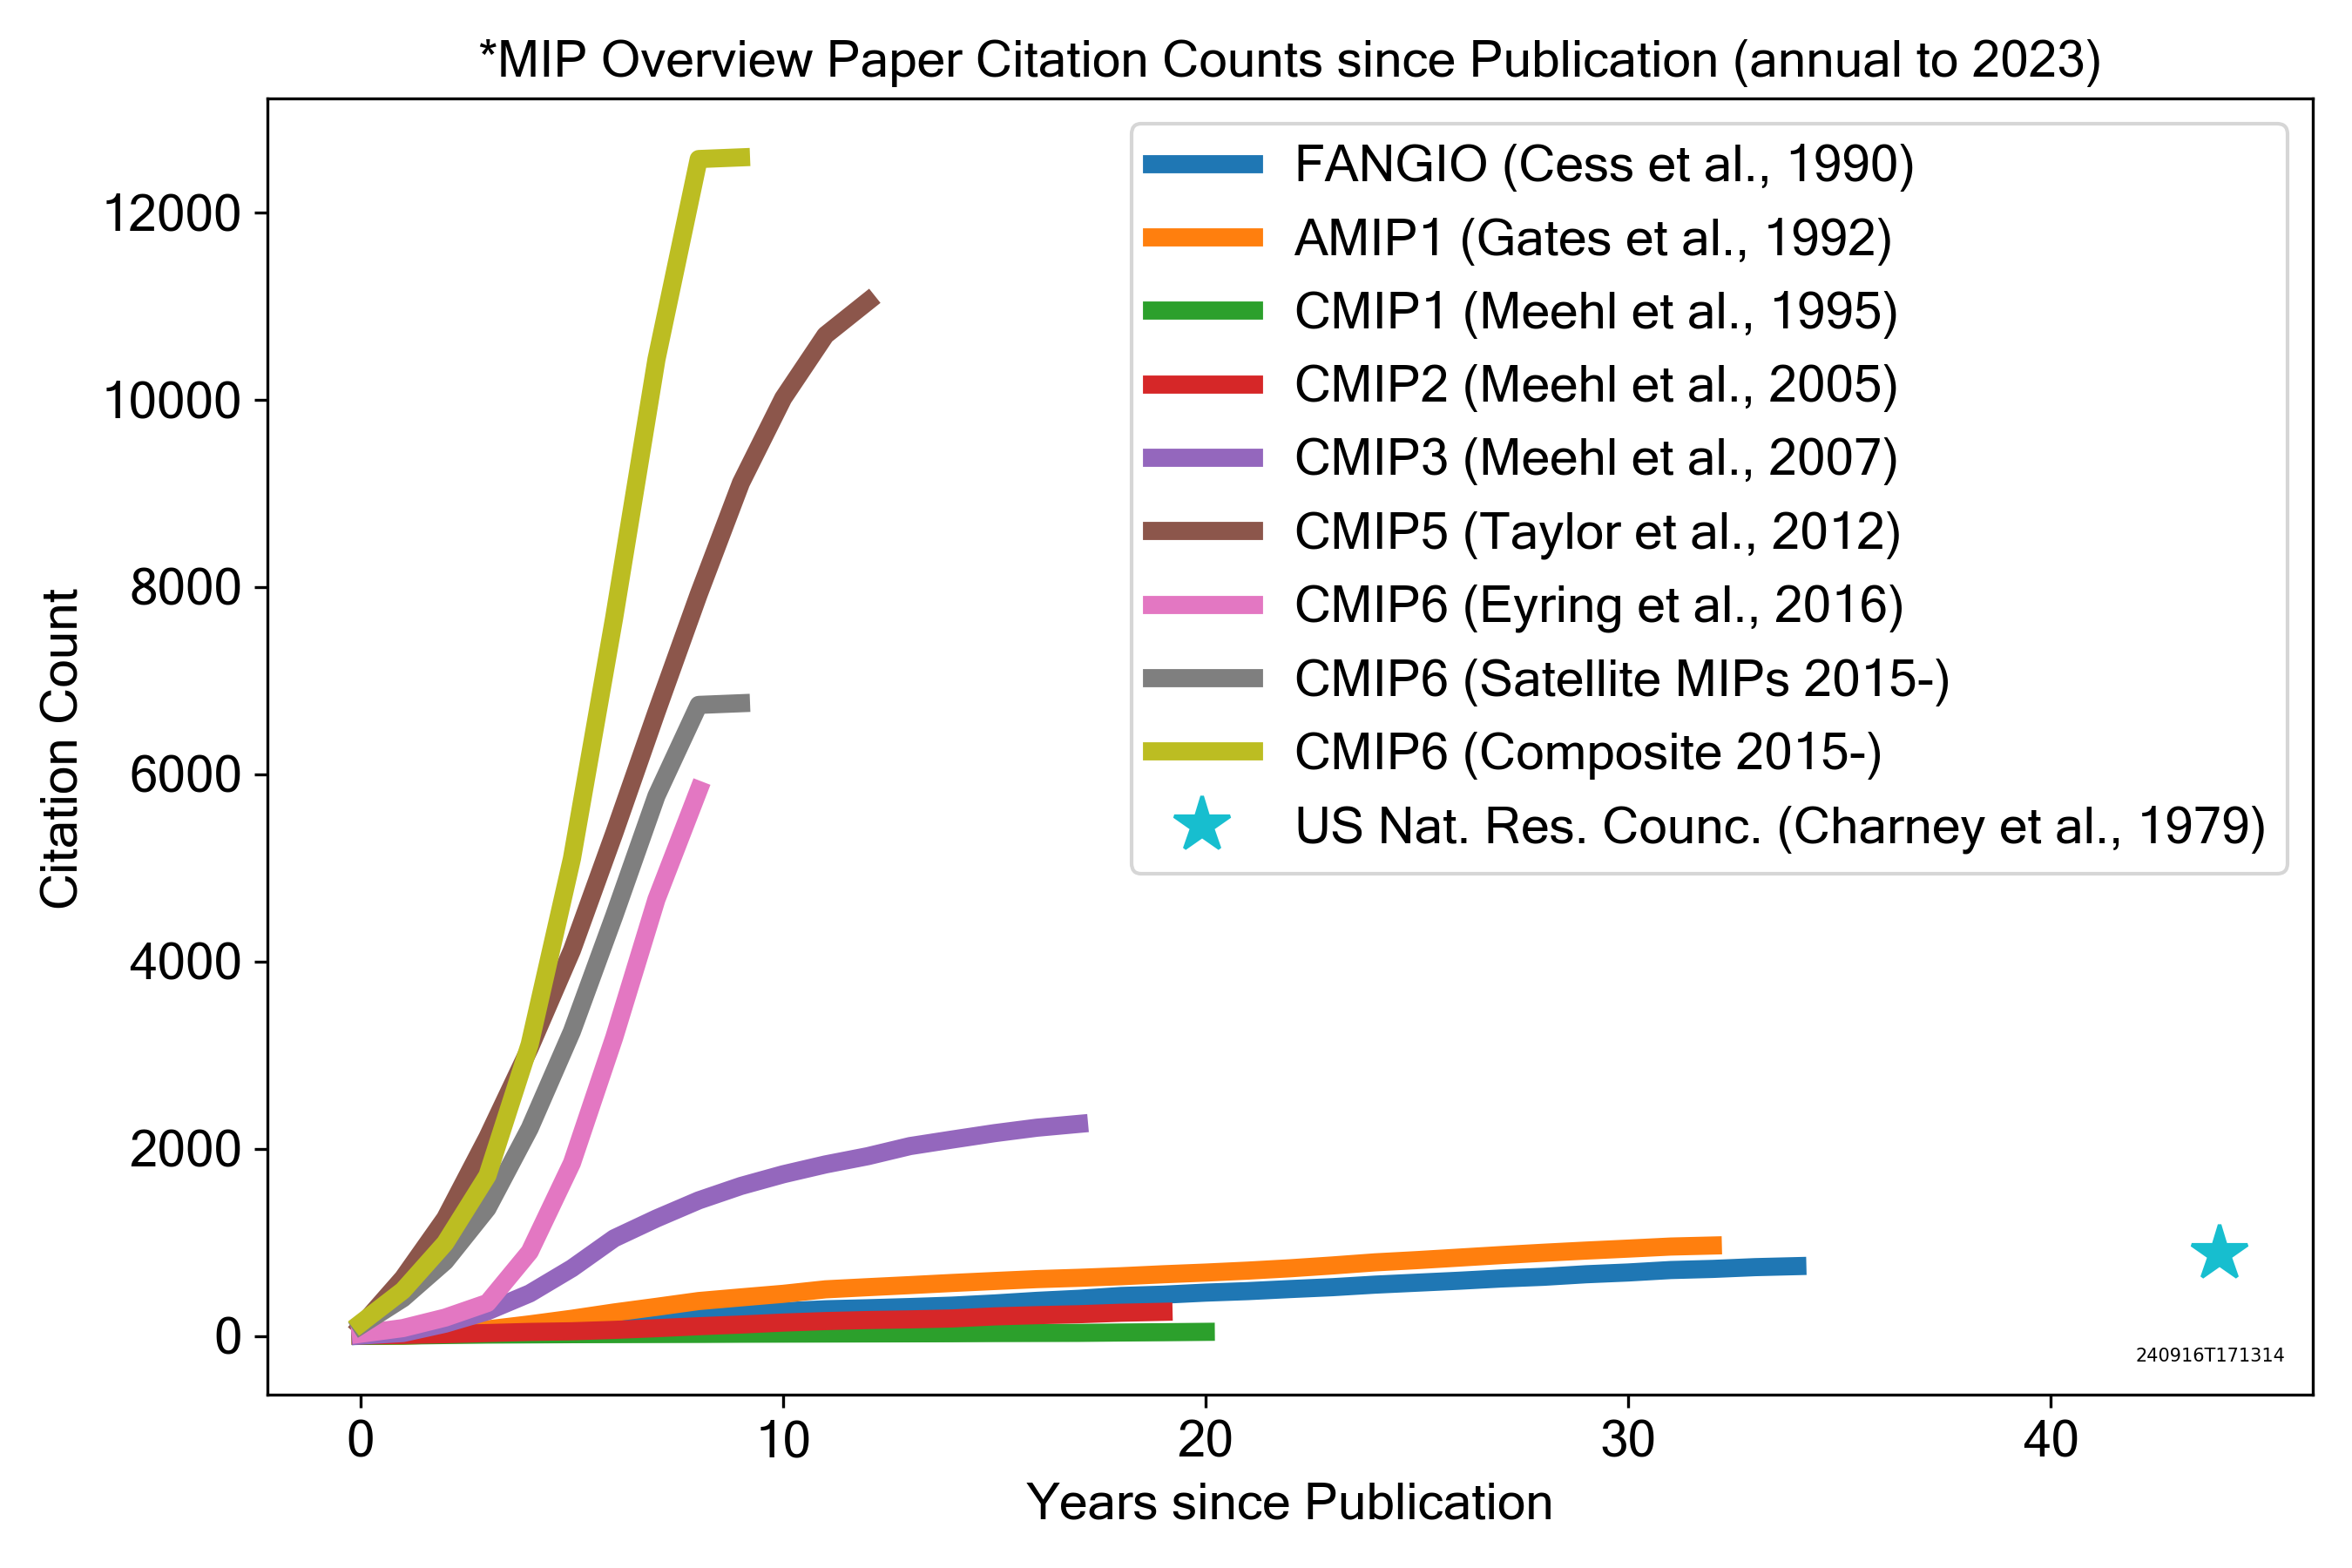
\includegraphics[width=1\linewidth]{240916T171314_CMIPOverviewPaperCitations-Counts-3.png}
    \caption{Web of Science citations for key overview papers of all MIP phases, from FANGIO \citep{cess_intercomparison_1990} through CMIP6, both the project overview paper \citep{eyring_overview_2016}, each of the community MIPs that comprise the phase (see \autoref{tab:tab2-CMIP6MIPs}) and a composite of these two sources from their publication to today. Citation counts are an imperfect way to capture MIP impact, but is reflective of a large and very strongly growing user community that has been using MIP data across the numerous phases. \cred{Update colour scheme to something more attractive, ala \autoref{fig:fig4-MIPCitations} colour scheme}}
    \label{fig:fig3-MIPPhaseCitations}
\end{figure}

% all figures and data should live in standalone github repo
\begin{figure*}
    \centering
    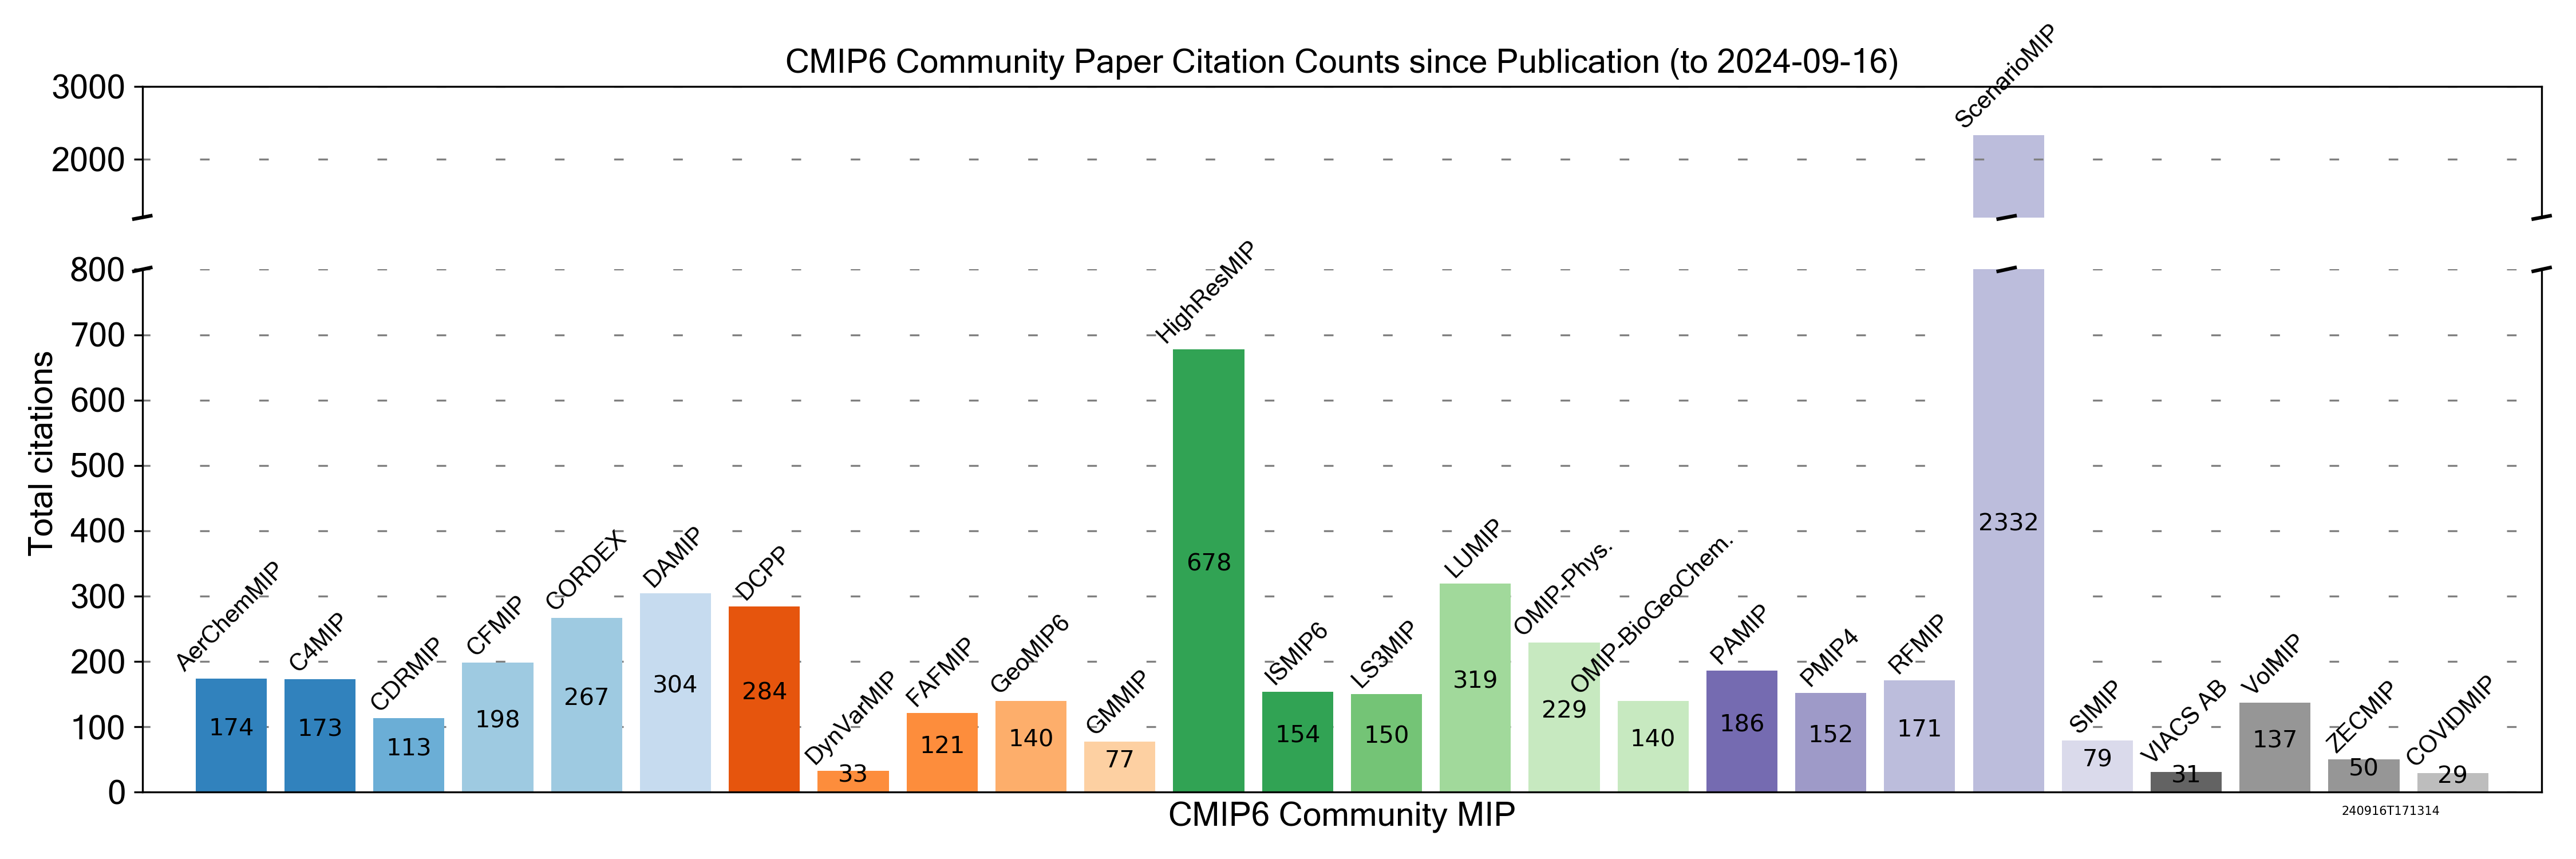
\includegraphics[width=\textwidth]{240916T171314_CMIPOverviewPaperCitations-Counts-2b-bar.png}
    \caption{Web of Science citations for the 23 MIPs contributing to CMIP6 (see \autoref{tab:tab2-CMIP6MIPs}) from their publication to today. Black text numbers on each coloured bar denote citation counts. Citation counts are an imperfect way to capture MIP impact, but is reflective of the large interest in the future climate change projections captured by ScenarioMIP \citep{oneill_scenario_2016}, and the high-resolution simulations captured in HighResMIP \citep{haarsma_high_2016}.}
    \label{fig:fig4-MIPCitations}
\end{figure*}

% all figures and data should live in standalone github repo
\begin{figure}
    \centering
    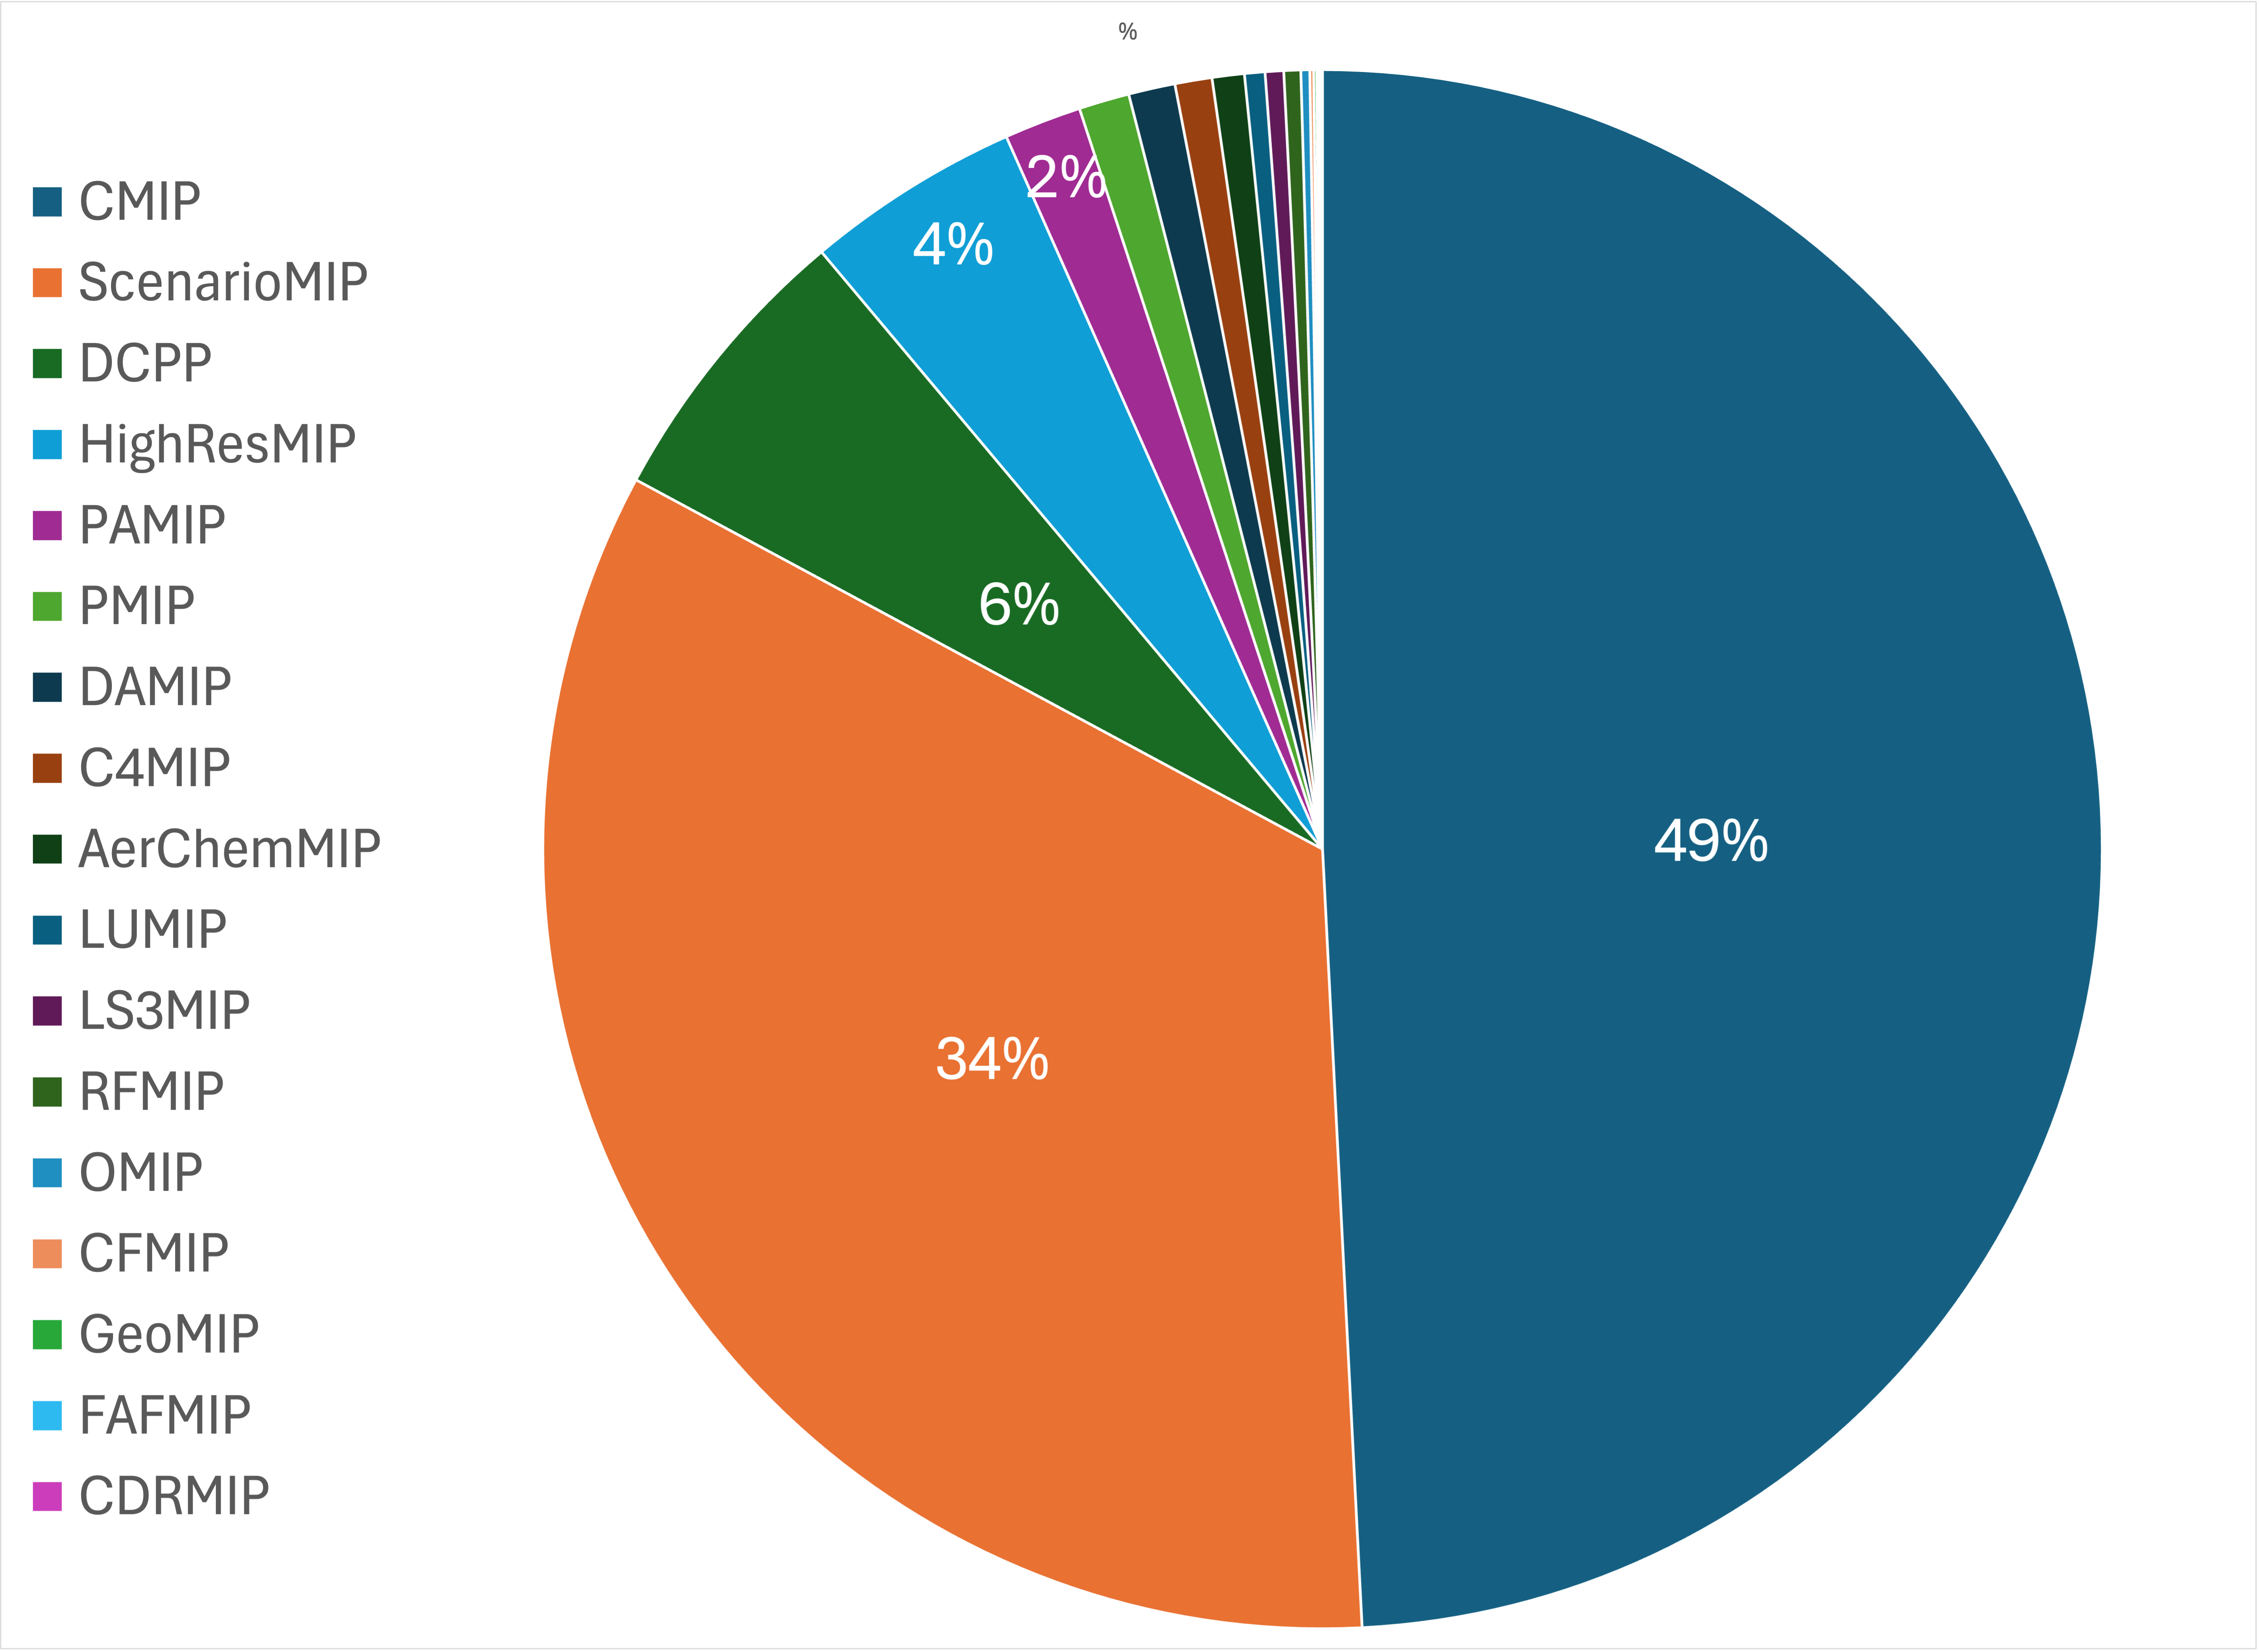
\includegraphics[width=1\linewidth]{240918_durack1-cmip6-experiments_240903.png}
    \caption{Recorded downloads across the 20 MIPs that have published data to ESGF (see \autoref{tab:tab2-CMIP6MIPs}). Almost 50\% of downloads were accounted for by the core CMIP/DECK simulations \citep{eyring_overview_2016}, with more than 30\% accounted for in the future projection experiments in ScenarioMIP \citep{oneill_scenario_2016}.}
    \label{fig:fig5-MIPDownloads}
\end{figure}

% all figures and data should live in standalone github repo
\begin{figure*}
    \centering
    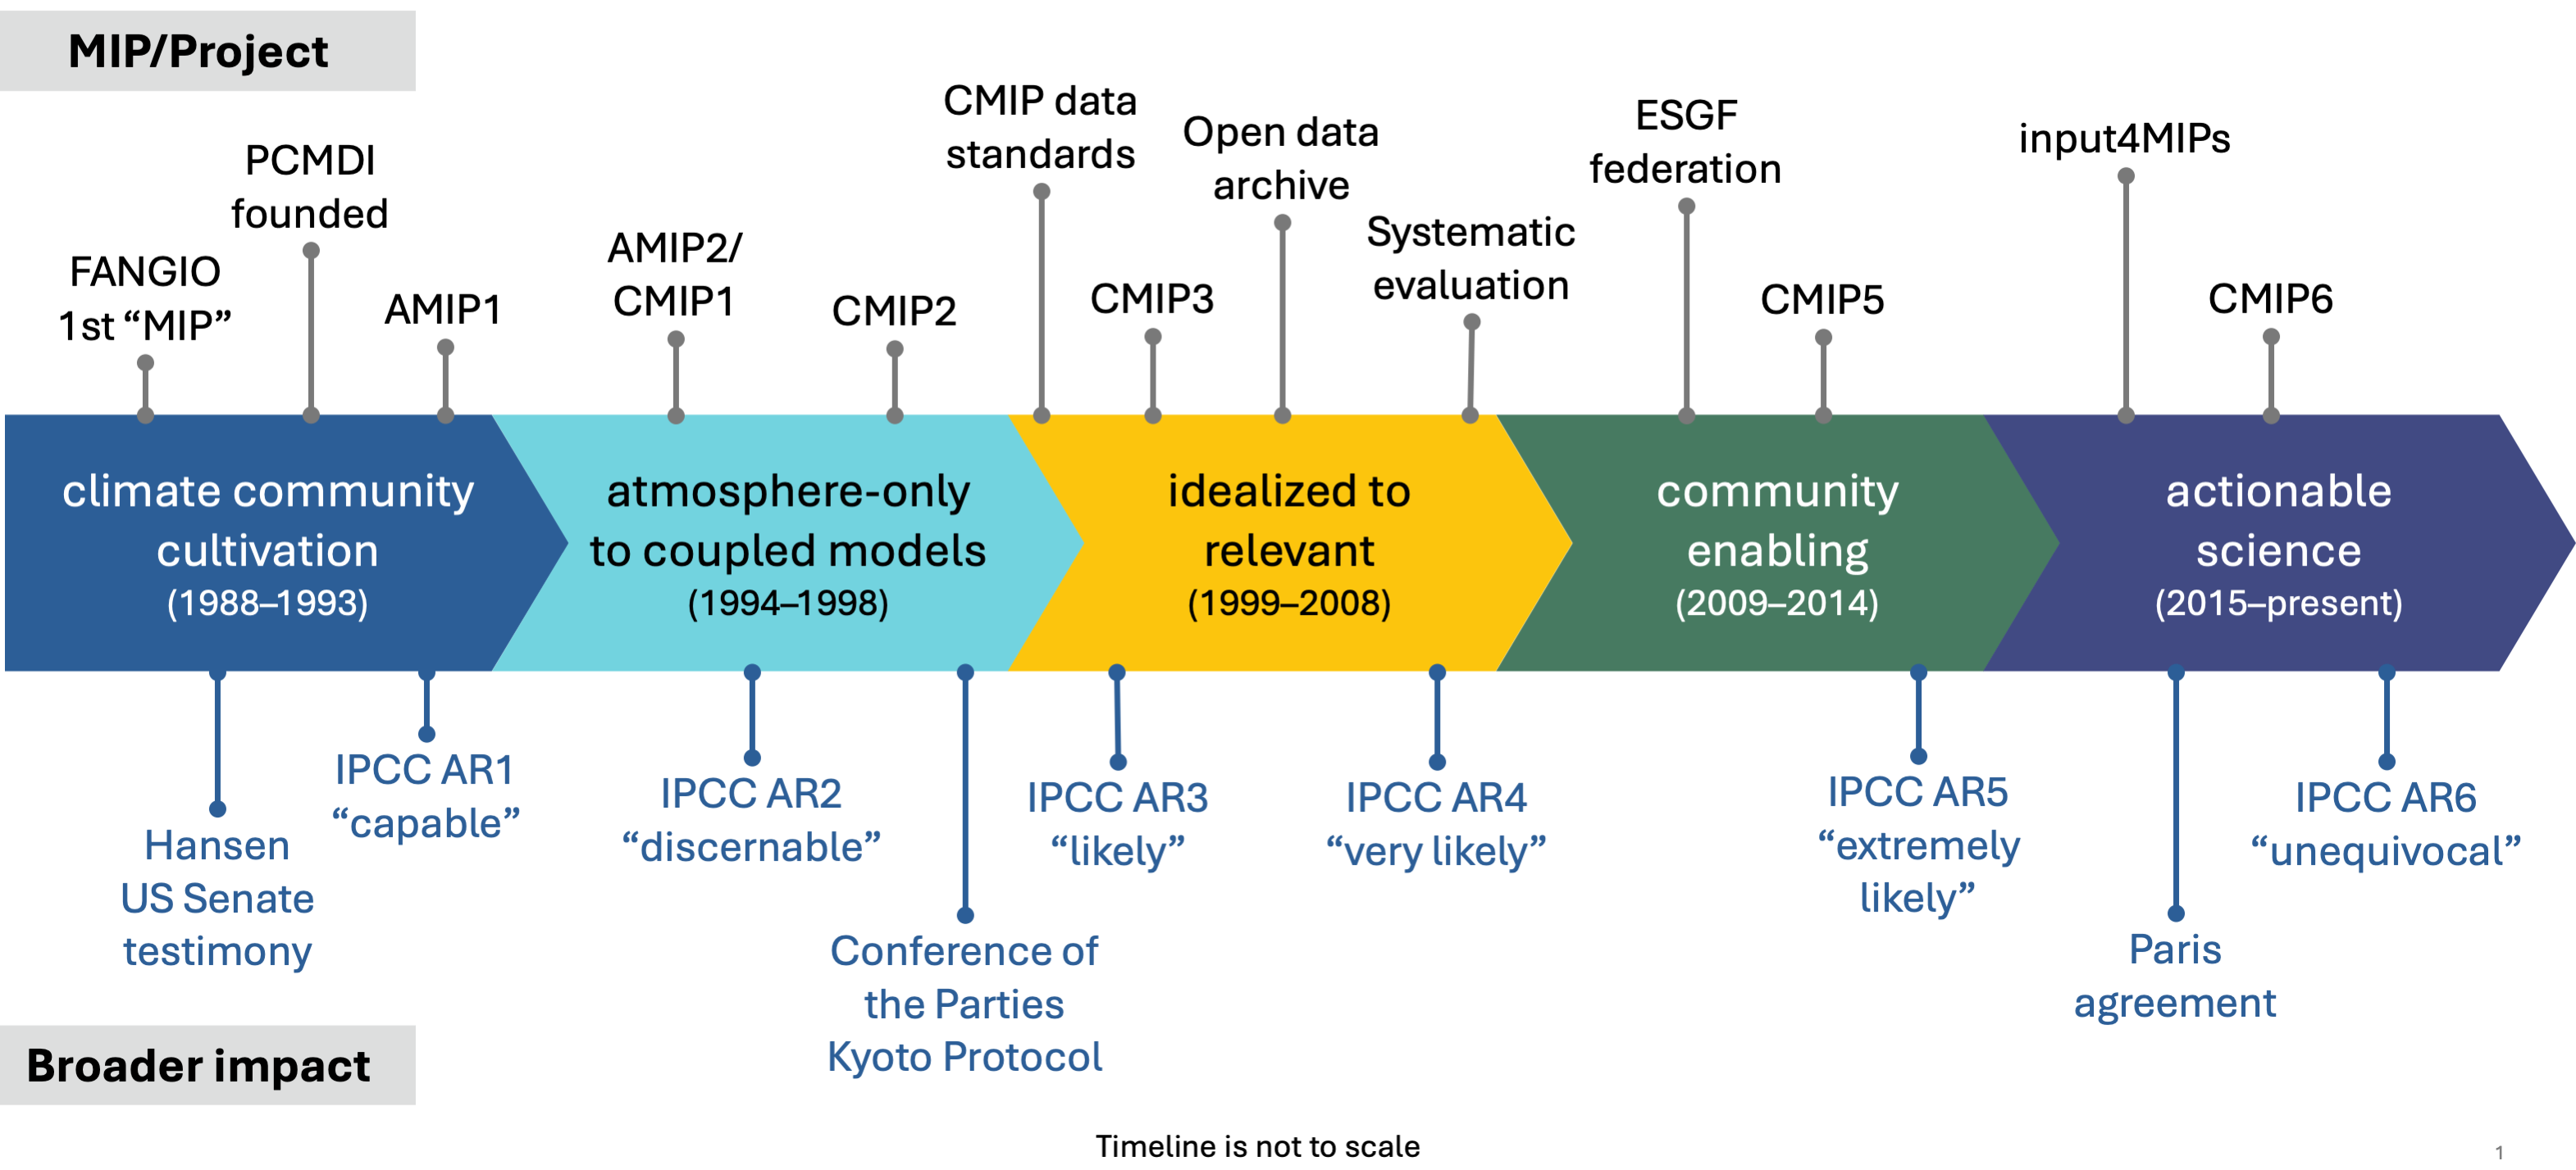
\includegraphics[width=\textwidth]{241019_durack1-AMIP-CMIP-IPCC-Impact-trim.png}
    \caption{A time history of MIPs and their broader impact, with particular relevance to the IPCC Assessment Report phases and statements of human influence on the climate (in parentheses, FAR through AR6; see \autoref{sec:amip1And2} through \autoref{sec:cmip6ProjectDesign}).}
    \label{fig:fig6-MIPImpact}
\end{figure*}


\section{CMIP6 impact and completion}
\label{sec:CMIP6Completion}
Planning is underway for a future CMIP7 phase, with the expectation that project data will become available in 2025. Following the CMIP6 broad expansion, CMIP7 will likely further federate discrete activities and encompass climate model simulations from an even broader contributor pool. Infrastructure providers are undertaking considerable updates to modernize the supporting hardware and software for project delivery to facilitate the transition. In preparation for the transition, continued publications to the CMIP6 archive will cease in early 2025, with the project sunsetting soon after that. CMIP6 data will continue to be made available through the federated ESGF network, however, the priority for data curation and maintenance will shift in favour of CMIP7 soon after the first datasets become available.

\cred{
\begin{itemize}
	\item Need for CMIP IPO identified in 2019 and open call for tenders
	\item CMIP IPO awarded 2021
	\item Aiding broad community engagement and formalization of governance allowing development of Task Teams to meet CMIP7 planning needs
	\item $\sim$35 MIPs self identified - see MIP rego page
	\item Broad community consultation
	\item Larger more coordinated activities
	\item Still dependent on infrastructure providers (engaged since CMIP3) to deliver the project
    \item Fresh eyes, early career engagement
\end{itemize}
}

\cred{GMD CMIP7 Special Issue; GMD CMIP7 Forcings Special Issue; Infrastructure concepts of multiverse/CMIP, planet/project and continent/user}



\section{Conclusions and next steps} %% \conclusions[modified heading if necessary]
\label{sec:Conclusions}
\cred{awaiting sections to be written above}

\cred{Would explicitly calling out the Stevens, 2024 and Jakobs et al., 2024 CMIP commentary papers make sense in this section}


%% Following commands are statements for data sets and/or software code availability corresponding to the manuscript.
%% Use these sections if data sets and/or software code are part of what your research article is based.

%\codeavailability{TEXT} %% use this section when having only software code available

%\dataavailability{TEXT} %% use this section when having only data sets available

\codedataavailability{github repos for data and figures} %% use this section when having data sets and software code available

%\sampleavailability{TEXT} %% use this section when having geoscientific samples available

%\videosupplement{TEXT} %% use this section when having video supplements available

\appendix
\section{Defined experiments across MIP phases}    %% Appendix A
%\subsection{}     %% Appendix A1, A2, etc.
\label{sec:secAppA1-MIPExperiments}
There is considerable continuity with experimental protocols across phases. The "amip" (atmosphere-only) experiment is where MIP science began, covering the 1979-1988 period for AMIP1, and 1979-2001 for AMIP2. The concept of a fixed climatological forced "control" experiment identified core experiments between CMIP1 and CMIP2, with the present-day control (pdcntrl, $\sim$1995 CMIP1) evolving to include a pre-industrial control (picntrl, $\sim$1850-1860 CMIP2) in subsequent phases. When assessing the "control" experiments, the nomenclature changed a little, with picntrl (before CMIP5) and piControl referring to the same experimental protocols, noting differing "pre-industrial" climatological fixed forcings were used across phases (see \autoref{sec:input4MIPs}). Idealized experiments were also incorporated in CMIP2, with the 1\% compounding (1pctCO2) first included and subsequently identified as 1pctto2x and 1pctto4x (before CMIP5), returning to the single 1pctCO2 identity in CMIP5 onward, and with differing simulation lengths across contributing models (2x 70 years, and 4x 140 years). The historical experiment, with transient time-evolving forcings included, was first defined in CMIP3, identified as 20C3M (climate of the twentieth century, $\sim$1860-1999). This is subsequently the historical experiment (CMIP5 and onward) and was extended to include additional forcing coverage (CMIP5: 1850-2011; CMIP6: 1850-2014). For further details and comparisons, see \autoref{tab:tabAppA1-MIPExperiments}, and to visualize the experiment growth over phases, see \autoref{fig:fig1-MIPGrowth}.

\begin{table*}[htp]
	\renewcommand{\arraystretch}{1.5}
	\scriptsize
	\centering
	\caption{MIP Experiments AMIP1 (1991) through CMIP6}
	\resizebox{\textwidth}{!} {
		\begin{tabularx}{0.9\textwidth} {
				| >{\centering\arraybackslash\hsize=.08\hsize}X
				| >{\centering\arraybackslash\hsize=.2\hsize}X
				| >{\centering\arraybackslash\hsize=.46\hsize}X
				| >{\centering\arraybackslash\hsize=.26\hsize}X | }
			\hline
			\textbf{MIP Phase} & \textbf{Citation/Year} & \textbf{Experiment(s)} & \textbf{URL/DOI}\\
			\hline
			AMIP1 & \citet{gates_amip_1991} & amip & 10.5281/zenodo.12109765; https://web.archive.org/web/ 19970524094021/http://www-pcmdi.llnl.gov/amip/\\
			\hline
			AMIP2 & \citet{gleckler_amip_1999} & amip & 10.5281/zenodo.12188729; https://web.archive.org/web/ 19970524094021/http://www-pcmdi.llnl.gov/amip/\\
			\hline
			CMIP1 & \citet{meehl_global_1995} & pdcntrl & https://web.archive.org/web/ 19970824235843/http://www-pcmdi.llnl.gov/cmip/Cmip.htm\\
			\hline
			CMIP2 & \citet{meehl_intercomparison_1997} & pdcntrl, picntrl, 1pctCO2 & https://web.archive.org/web/ 19970825000210/http://www-pcmdi.llnl.gov/cmip/announ.htm\\
			\hline
			CMIP3 & Doutriaux \& Taylor, 2005; \citet{meehl_wcrp_2007} & 1pctto2x, 1pctto4x, 20c3m, amip, commit, pdcntrl, picntrl; \textbf{CFMIP:} 2xco2, slabcntl; \textbf{ScenarioMIP:} sresa1b, sresa2, sresb1 & https://pcmdi.llnl.gov/mips/ cmip3/experiment.html\#Experiments\\
			\hline
			CMIP5 & \cite{taylor_overview_2012}; Doutriaux \& Taylor, 2013 & 1pctCO2, abrupt4xCO2, amip, historical, piControl; \textbf{C4MIP:} esmControl, esmFdbk1, esmFdbk2, esmFixClim1, esmFixClim2, esmHistorical, esmrcp85; \textbf{CFMIP:} amip4K, amip4xCO2, amipFuture, aqua4K, aqua4xCO2, aquaControl, sst2030; \textbf{DCPP:} decadalXXXX, noVolcXXXX, volcIn2010; \textbf{DAMIP:} historicalExt, historicalGHG, historicalMisc, historicalNat; \textbf{PMIP:} lgm, midHolocene, past1000; \textbf{RFMIP:} sstClim, sstClim4xCO2, sstClimAerosol, sstClimSulfate; \textbf{ScenarioMIP:} rcp26, rcp45, rcp60, rcp85 & https://pcmdi.llnl.gov/mips/ cmip5/experiment\_design.html\\
			\hline			
			CMIP6 & \citet{eyring_overview_2016}; Durack et al., 2024 & see CMIP6\_CVs; for MIPs contributing to the phase see \autoref{tab:tab2-CMIP6MIPs} & https://github.com/WCRP-CMIP/CMIP6\_CVs; https://wcrp-cmip.github.io/CMIP6\_CVs/ docs/CMIP6\_experiment\_id.html\\
			\hline		
		\end{tabularx}
	} % /resizebox
	\label{tab:tabAppA1-MIPExperiments}
	\text{Note numbers are calculated in an excel spreadsheet for the early text or web-based lists}
 % Mappings see Taylor google doc XML filename construction https://docs.google.com/document/d/1bUwK6G_fVZO53UjLZbQUOuBP47PsT8lqKKhL1pjRnKg/edit
\end{table*}


\section{MIP standard outputs}    %% Appendix B
\label{sec:secAppB1-MIPStandardOutput}
The information presented in \autoref{tab:tab1-MIPsThroughTime} row "Standard output variables/Tables" was collated from numerous live and archived resources available from 1991 through to the CMIP6 CMOR Table files that are still being used today. The earliest resources were published in written form, the AMIP Newsletters (e.g., \citet{gates_amip_1991}), and subsequently, became available on the PCMDI website for AMIP2, CMIP1 and CMIP2/2+ phases. CMIP3 marked a step change, with the development of the CMOR1 software (\citet{taylor_cmor_2006}) and CMIP3 Standard Output defined by the more complete CMIP3-CMOR-Tables (\citet{doutriaux_cmip3_2005}). CMIP5 continued this trend with CMOR2 (\citet{doutriaux_cmor_2011}) and the CMIP5-CMOR-Tables (\citet{doutriaux_cmip5_2013}). For CMIP6, project expansion to include 23 MIPs and 322 experiments (\autoref{tab:tab2-CMIP6MIPs}, \autoref{tab:tab1-MIPsThroughTime} respectively) required the development of a dedicated CMIP6 Data Request (see \autoref{sec:CMIP6DR}) along with the parallel development of CMOR3 (\citet{mauzey_cmor_2024}) and the CMIP6-CMOR-Tables (\citet{nadeau_cmip6_2017}). For each tabulated value, superscript-identified links provide live connections to these sources.

\begin{table*}[htp]
	\renewcommand{\arraystretch}{1.5}
	\scriptsize
	\centering
	\caption{MIP standard output AMIP1 (1991) to CMIP6}
	\resizebox{\textwidth}{!} {
		\begin{tabularx}{0.9\textwidth} {
				| >{\centering\arraybackslash\hsize=.09\hsize}X
				| >{\centering\arraybackslash\hsize=.09\hsize}X
				| >{\centering\arraybackslash\hsize=.09\hsize}X
                | >{\centering\arraybackslash\hsize=.1\hsize}X
				| >{\centering\arraybackslash\hsize=.63\hsize}X | }
			\hline
			\textbf{Table 1 superscript} & \textbf{MIP Phase} & CMOR version & \textbf{Citation/Year} & \textbf{URL/DOI}\\
			\hline
			1 & AMIP1 & $\sim$ & \citet{gates_amip_1991} & 10.5281/zenodo.12109765; https://pcmdi.llnl.gov/mips/amip/OUTPUT/WGNEDIAGS/index.html?\\
			\hline
			2 & AMIP2 & $\sim$ & 1998 & https://pcmdi.llnl.gov/mips/amip/OUTPUT/AMIP2/outlist.html\\
			\hline
			3 & CMIP1 & $\sim$ & 1997 & https://web.archive.org/web/19970824233750/http://www-pcmdi.llnl.gov/cmip/diagsub.html\\
			\hline
			4 & CMIP2 & $\sim$ & 1997 & https://pcmdi.llnl.gov/mips/cmip2/\\
			\hline
			5 & CMIP3 & 1.0 & Doutriaux \& Taylor, 2005 & 10.5281/zenodo.12792173; https://github.com/PCMDI/cmip3-cmor-tables\\ \hline
			6 & CMIP5 & 2.0 & Doutriaux \& Taylor, 2013 & 10.5281/zenodo.12792191; https://github.com/PCMDI/cmip5-cmor-tables\\ \hline
			7 & CMIP6 & 3.0 & Nadeau et al., 2018 & 10.5281/zenodo.597650; https://github.com/PCMDI/cmip6-cmor-tables\\
			\hline
			\hline
			$\sim$ & CFMIP1 & 1.0 & $\sim$ & https://github.com/PCMDI/cfmip1-cmor-tables\\
			\hline
			$\sim$ & C-LAMP1 & 1.0 & $\sim$ & https://github.com/PCMDI/c-lamp1-cmor-tables/\\
			\hline
			$\sim$ & IAEMIP1 & 1.0 & $\sim$ & https://github.com/PCMDI/iaemip1-cmor-tables\\
			\hline
            $\sim$ & CORDEX & 2.0 & $\sim$ & https://github.com/PCMDI/cordex-cmor-tables\\
			\hline
			$\sim$ & GEOMIP & 2.0 & $\sim$ & https://github.com/PCMDI/geomip-cmor-tables\\
			\hline
			$\sim$ & LUCID & 2.0 & $\sim$ & https://github.com/PCMDI/lucid-cmor-tables\\
			\hline
			$\sim$ & PMIP3 & 2.0 & $\sim$ & https://github.com/PCMDI/pmip3-cmor-tables\\
			\hline
			$\sim$ & CORDEX-CMIP6 & 3.0 & \citet{gutowski_jr_wcrp_2016} & https://github.com/WCRP-CORDEX/cordex-cmip6-cmor-tables\\
            \hline
			others? & $\sim$ & $\sim$ & $\sim$ & $\sim$\\
			\hline
        \end{tabularx}
	} % /resizebox
	\label{tab:tabAppB1-MIPStandardOutput}
	\text{}
\end{table*}


\section{MIP errata}    %% Appendix C
\label{sec:secAppC1-MIPErrata}
Tabulated entries of CMIP errata based on phase

\begin{table*}[htp]
	\renewcommand{\arraystretch}{1.5}
	\scriptsize
	\centering
	\caption{MIP Errata CMIP3 (2004) to CMIP6}
	\resizebox{\textwidth}{!} {
		\begin{tabularx}{0.9\textwidth} {
				| >{\centering\arraybackslash\hsize=.1\hsize}X
				| >{\centering\arraybackslash\hsize=.25\hsize}X
				| >{\centering\arraybackslash\hsize=.65\hsize}X | }
			\hline
			\textbf{MIP Phase} & \textbf{Errata count (reporting period)} & \textbf{URL/DOI}\\ \hline
			CMIP3 & 122 (2004-2011) & http://web.archive.org/web/20150906073117/https://esg.llnl.gov:8443/about/errata.do\\ \hline
			CMIP5 & 84 (2012-2015) & https://pcmdi.llnl.gov/mips/cmip5/errata.html\\ \hline
			CMIP6 & 492 (2018-2024) & https://errata.ipsl.fr\\
			\hline
		\end{tabularx}
	} % /resizebox
	\label{tab:tabAppC1-MIPErrata}
	\text{Note: All values are tabulated from archived or live webpages as of \DTMsetstyle{en-GB}\DTMnow}
\end{table*}

\mycomment{
What do we need DOI'd - can zenodo work?
CMIP2: https://pcmdi.llnl.gov/mips/cmip2/
CMIP3: https://pcmdi.llnl.gov/mips/cmip3/experiment.html
CMIP5: https://pcmdi.llnl.gov/mips/cmip5/requirements.html
standard_output doc - with coverpage (Karl)
ODS2.5: Gleckler et al. 2024 https://docs.google.com/document/d/1bTi5-CKR8xBCA4e3egc4FXJ93LuUfrhyEBHpUCVgZuo/edit
Also Potter et al. 2011 https://doi.org/10.1175/2011BAMS3018.1
}


\section{CMIP6 data preparation tools}    %% Appendix D
\label{sec:secAppD1-CMIP6DataPrep}

During MIP phases, several software tools have been developed and updated to meet augmented phase requirements. These tools build on the MIP nomenclature and digital formats that are now standard. Some key packages are tabulated below (see \autoref{tab:tab3-CMIPSoftware}).

\begin{table*}[htp]
\renewcommand{\arraystretch}{2}
\scriptsize
\centering
\caption{Software packages developed to aid MIP dataset production}
\resizebox{\textwidth}{!} {
	\begin{tabularx}{0.9\textwidth} { 
	  | >{\raggedright\arraybackslash\hsize=.14\hsize}X
	  | >{\centering\arraybackslash\hsize=.2\hsize}X
	  | >{\centering\arraybackslash\hsize=.46\hsize}X
	  | >{\centering\arraybackslash\hsize=.1\hsize}X
	  | >{\centering\arraybackslash\hsize=.1\hsize}X | }
\hline
\textbf{Software name and version} & \textbf{Software Description} & \textbf{URL} & \textbf{Citation} & \textbf{DOI} \\
\hline
CMOR 1.0 & The Climate Model Output Rewriter & https://cmor.llnl.gov/archive/cmor1/, https://github.com/PCMDI/cmor & \citet{taylor_cmor_2006} & 10.5281/ zenodo.12690071 \\
\hline
CMOR 2.0 & The Climate Model Output Rewriter & https://cmor.llnl.gov, https://github.com/PCMDI/cmor & \citet{doutriaux_cmor_2011} & 10.5281/ zenodo.12690366 \\
\hline
CMOR 3.0 & The Climate Model Output Rewriter & https://cmor.llnl.gov, https://github.com/PCMDI/cmor & \citet{doutriaux_cmor_2024} & 10.5281/ zenodo.592733 \\
\hline
XIOS & Xml IO Server & http://forge.ipsl.jussieu.fr/ioserver/chrome/site/XIOS\_DOC &  &  \\
\hline
ECE2CMOR3 & EC-Earth to CMOR & https://github.com/EC-Earth/ece2cmor3, https://github.com/EC-Earth/cmor-fixer &  & 10.5281/ zenodo.1051094 \\
\hline
CDO CMOR & Climate Data Operators to CMOR & https://code.mpimet.mpg.de/projects/cdo/wiki/ CDO\_CMOR\_Operator &  &  \\
\hline
NORESM2CMOR & NorESM to CMOR & https://github.com/NorESMhub/noresm2cmor &  &  \\
\hline
CCLM2CMOR & COSMO-CLM to CMOR & https://github.com/C2SM-RCM/CCLM2CMOR, https://github.com/ssilje/CMOR &  &  \\
\hline
FGOALS-g-cmor & FGOALS-g to CMOR & https://github.com/dongli/FGOALS-g-cmor &  &  \\
\hline
PRIMAVERA & HadGEM to CMOR & https://github.com/goord/cmor &  &  \\
\hline
E3SM\_To\_CMIP & DOE-E3SM to CMOR & https://github.com/E3SM-Project/e3sm\_to\_cmip &  &  \\
\hline
\end{tabularx}
} % /resizebox
\label{tab:tab3-CMIPSoftware}
\end{table*}


\noappendix       %% use this to mark the end of the appendix section. Otherwise, the figures might be numbered incorrectly (e.g., 10 instead of 1).

%% Regarding figures and tables in appendices, the following two options are possible depending on your general handling of figures and tables in the manuscript environment:

%% Option 1: If you sorted all figures and tables into the text sections, please also sort the appendix figures and appendix tables into the respective appendix sections.
%% They will be correctly named automatically.

%% Option 2: If you put all figures after the reference list, please insert appendix tables and figures after the normal ones.
%% To rename them correctly to A1, A2, etc., please add the following commands in front of them:

\appendixfigures  %% needs to be added in front of appendix figures

\appendixtables   %% needs to be added in front of the appendix tables

%% Please add \clearpage between each table and/or figure. Further guidelines on figures and tables can be found below.



\authorcontribution{P.J.D. outlined the content, completed the initial outline, and shared responsibility for writing the manuscript. K.E.T. assisted in expanding the outline and shared responsibility for writing the manuscript. P.J.G. provided useful feedback on early drafts. All authors contributed to the final version of the manuscript.} %% This section is mandatory

\competinginterests{All authors declare no competing or conflicting interests} %% this section is mandatory even if you declare that no competing interests are present

\disclaimer{TEXT} %% optional section

\begin{acknowledgements}

We acknowledge all MIP contributing modelling groups, the World Climate Research Programmes (WCRP) Working Group on Coupled Modelling (WGCM) and its WGCM Infrastructure (WIP) and the CMIP Panels for their leadership in defining and delivering multiple CMIP and preceding AMIP phases. We acknowledge the Program for Climate Model Diagnosis and Intercomparison (PCMDI, USA), Centre for Environmental Data Analysis (CEDA, UK), the German Climate Computing Centre (DKRZ, Germany), the Institute Pierre-Simon Laplace (IPSL, France), Centro Euro-Mediterraneo sui Cambiamenti Climatici (CMCC, Italy), the Earth System Grid Federation (ESGF) and Earth System Grid (ESG) contributing organizations and many other infrastructure providers for developing the ecosystem that delivered MIP data across multiple phases. The U.S. Department of Energy supports P.J.D., K.E.T., P.J.G., and J.L. from Lawrence Livermore National Laboratory under contract DE-AC52-07NA27344.

We thank numerous colleagues, collaborators, and past contributors to CMIP for their valuable input and feedback.

We acknowledge three anonymous reviewers for helpful feedback on the initial draft, which strongly improved the manuscript.
\end{acknowledgements}


%% REFERENCES

%% The reference list is compiled as follows:

%\begin{thebibliography}{}
%\bibitem[AUTHOR(YEAR)]{LABEL1}
%REFERENCE 1
%\end{thebibliography}
\bibliographystyle{copernicus}
\bibliography{241025b}

%% Since the Copernicus LaTeX package includes the BibTeX style file copernicus.bst,
%% authors experienced with BibTeX only have to include the following two lines:
%%
%% \bibliographystyle{copernicus}
%% \bibliography{example.bib}
%%
%% URLs and DOIs can be entered in your BibTeX file as:
%%
%% URL = {http://www.xyz.org/~jones/idx_g.htm}
%% DOI = {10.5194/xyz}


%% LITERATURE CITATIONS
%%
%% command                        & example result
%% \citet{jones90}|               & Jones et al. (1990)
%% \citep{jones90}|               & (Jones et al., 1990)
%% \citep{jones90,jones93}|       & (Jones et al., 1990, 1993)
%% \citep[p.~32]{jones90}|        & (Jones et al., 1990, p.~32)
%% \citep[e.g.,][]{jones90}|      & (e.g., Jones et al., 1990)
%% \citep[e.g.,][p.~32]{jones90}| & (e.g., Jones et al., 1990, p.~32)
%% \citeauthor{jones90}|          & Jones et al.
%% \citeyear{jones90}|            & 1990



%% FIGURES

%% When figures and tables are placed at the end of the MS (article in one-column style), please add \clearpage
%% between bibliography and first table and/or figure and between each table and/or figure.

% The figure files should be labelled correctly with Arabic numerals (e.g. fig01.jpg, fig02.png).


%% ONE-COLUMN FIGURES

%%f
%\begin{figure}[t]
%\includegraphics[width=8.3cm]{FILE NAME}
%\caption{TEXT}
%\end{figure}
%
%%% TWO-COLUMN FIGURES
%
%%f
%\begin{figure*}[t]
%\includegraphics[width=12cm]{FILE NAME}
%\caption{TEXT}
%\end{figure*}
%
%
%%% TABLES
%%%
%%% The different columns must be seperated with a & command and should
%%% end with \\ to identify the column brake.
%
%%% ONE-COLUMN TABLE
%
%%t
%\begin{table}[t]
%\caption{TEXT}
%\begin{tabular}{column = lcr}
%\tophline
%
%\middlehline
%
%\bottomhline
%\end{tabular}
%\belowtable{} % Table Footnotes
%\end{table}
%
%%% TWO-COLUMN TABLE
%
%%t
%\begin{table*}[t]
%\caption{TEXT}
%\begin{tabular}{column = lcr}
%\tophline
%
%\middlehline
%
%\bottomhline
%\end{tabular}
%\belowtable{} % Table Footnotes
%\end{table*}
%
%%% LANDSCAPE TABLE
%
%%t
%\begin{sidewaystable*}[t]
%\caption{TEXT}
%\begin{tabular}{column = lcr}
%\tophline
%
%\middlehline
%
%\bottomhline
%\end{tabular}
%\belowtable{} % Table Footnotes
%\end{sidewaystable*}
%
%
%%% MATHEMATICAL EXPRESSIONS
%
%%% All papers typeset by Copernicus Publications follow the math typesetting regulations
%%% given by the IUPAC Green Book (IUPAC: Quantities, Units and Symbols in Physical Chemistry,
%%% 2nd Edn., Blackwell Science, available at: http://old.iupac.org/publications/books/gbook/green_book_2ed.pdf, 1993).
%%%
%%% Physical quantities/variables are typeset in italic font (t for time, T for Temperature)
%%% Indices which are not defined are typeset in italic font (x, y, z, a, b, c)
%%% Items/objects which are defined are typeset in roman font (Car A, Car B)
%%% Descriptions/specifications which are defined by itself are typeset in roman font (abs, rel, ref, tot, net, ice)
%%% Abbreviations from 2 letters are typeset in roman font (RH, LAI)
%%% Vectors are identified in bold italic font using \vec{x}
%%% Matrices are identified in bold roman font
%%% Multiplication signs are typeset using the LaTeX commands \times (for vector products, grids, and exponential notations) or \cdot
%%% The character * should not be applied as multiplication sign
%
%
%%% EQUATIONS
%
%%% Single-row equation
%
%\begin{equation}
%
%\end{equation}
%
%%% Multiline equation
%
%\begin{align}
%& 3 + 5 = 8\\
%& 3 + 5 = 8\\
%& 3 + 5 = 8
%\end{align}
%
%
%%% MATRICES
%
%\begin{matrix}
%x & y & z\\
%x & y & z\\
%x & y & z\\
%\end{matrix}
%
%
%%% ALGORITHM
%
%\begin{algorithm}
%\caption{...}
%\label{a1}
%\begin{algorithmic}
%...
%\end{algorithmic}
%\end{algorithm}
%
%
%%% CHEMICAL FORMULAS AND REACTIONS
%
%%% For formulas embedded in the text, please use \chem{}
%
%%% The reaction environment creates labels including the letter R, i.e. (R1), (R2), etc.
%
%\begin{reaction}
%%% \rightarrow should be used for normal (one-way) chemical reactions
%%% \rightleftharpoons should be used for equilibria
%%% \leftrightarrow should be used for resonance structures
%\end{reaction}
%
%
%%% PHYSICAL UNITS
%%%
%%% Please use \unit{} and apply the exponential notation


\end{document}
